\chapter{RESULTADOS E DISCUSSÃO}
Este capítulo detalha os resultados alcançados por meio da análise de sensibilidade aplicada às simulações no estudo do controle de trajetória em impressoras 3D. Essa análise é essencial para avaliar a eficiência do método de controle proposto, considerando sua resposta diante de diferentes condições e parâmetros operacionais. Os resultados destacam a robustez e a viabilidade do método em um contexto real de operação, ao mesmo tempo em que apontam suas possíveis limitações. A apresentação e interpretação dos dados têm como objetivo enfatizar o desempenho do método e oferecer percepções valiosas para futuros avanços e aplicações práticas na área de controle de trajetória para a manufatura aditiva.

Prosseguindo, a análise dos resultados inicia-se com a avaliação da simulação base, estabelecendo um ponto de referência para comparação. Em seguida, detalhamos o impacto e as implicações de cada um dos cinco parâmetros escolhidos na análise de sensibilidade. Estes parâmetros foram criteriosamente selecionados com o objetivo de explorar diferentes aspectos do método de controle e sua resposta em variados cenários operacionais. A investigação destes parâmetros oferece uma visão abrangente sobre como cada elemento influencia o desempenho geral do sistema, permitindo uma compreensão mais profunda e um refinamento do método proposto.

\section{Resultados da Simulação Referência}
Esta seção aborda os resultados obtidos na simulação de referência, com ênfase nas representações gráficas e na metodologia aplicada.

Análise de Velocidades (Figura \ref{fig:t_padr_vels}): Este gráfico exibe as variações das velocidades ao longo do tempo nos eixos X e Y. Ele demonstra a resposta dinâmica tanto da ponta do manipulador quanto da referência estabelecida, conforme a metodologia proposta.

\begin{figure}[H]
    \begin{center}
    \caption{Caso referência - Comportamento no tempo das velocidades em x e y da ponta e da referência}
    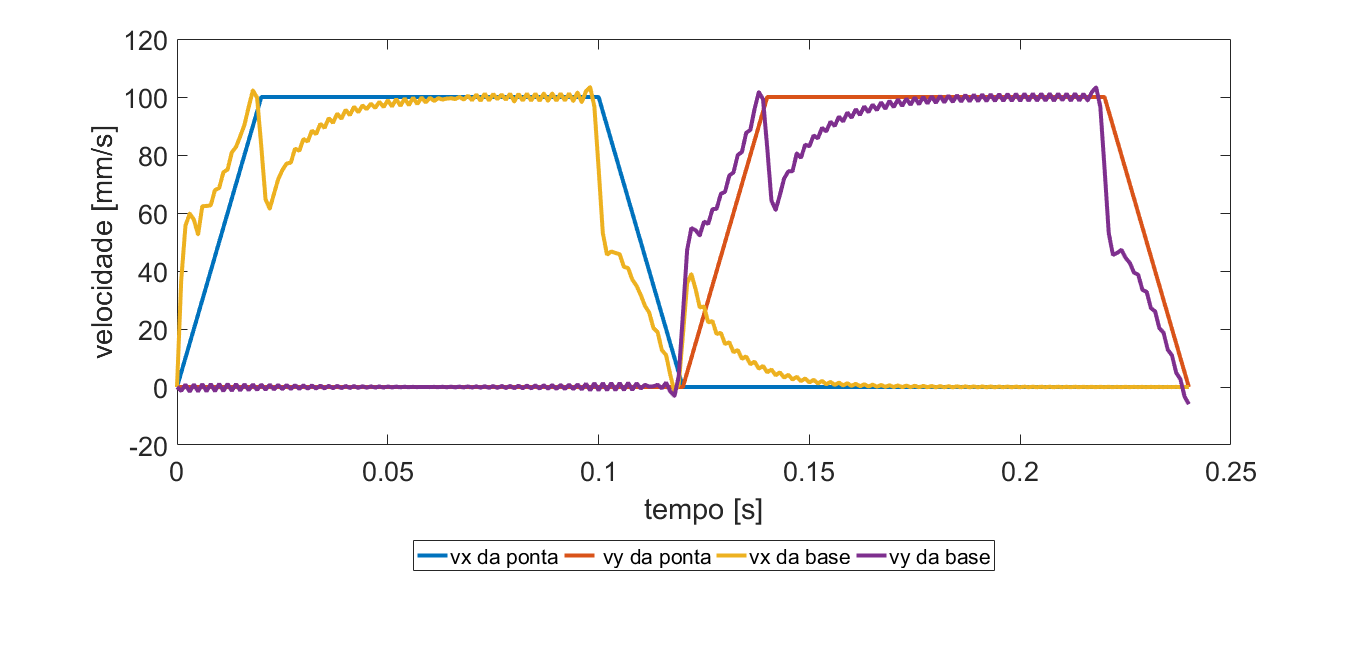
\includegraphics[scale=0.44]{Teste Padrao vels}
    \label{fig:t_padr_vels}
    \end{center}
\end{figure}

Deslocamentos Temporais (Figura \ref{fig:t_padr_des}): Aqui, os deslocamentos nos eixos X e Y são plotados contra o tempo. Esses resultados refletem diretamente a precisão e eficiência do sistema simulado, conforme os critérios estabelecidos na metodologia.

\begin{figure}[H]
    \begin{center}
    \caption{Caso referência - Comportamento no tempo dos deslocamentos em x e y da ponta e da referência}
    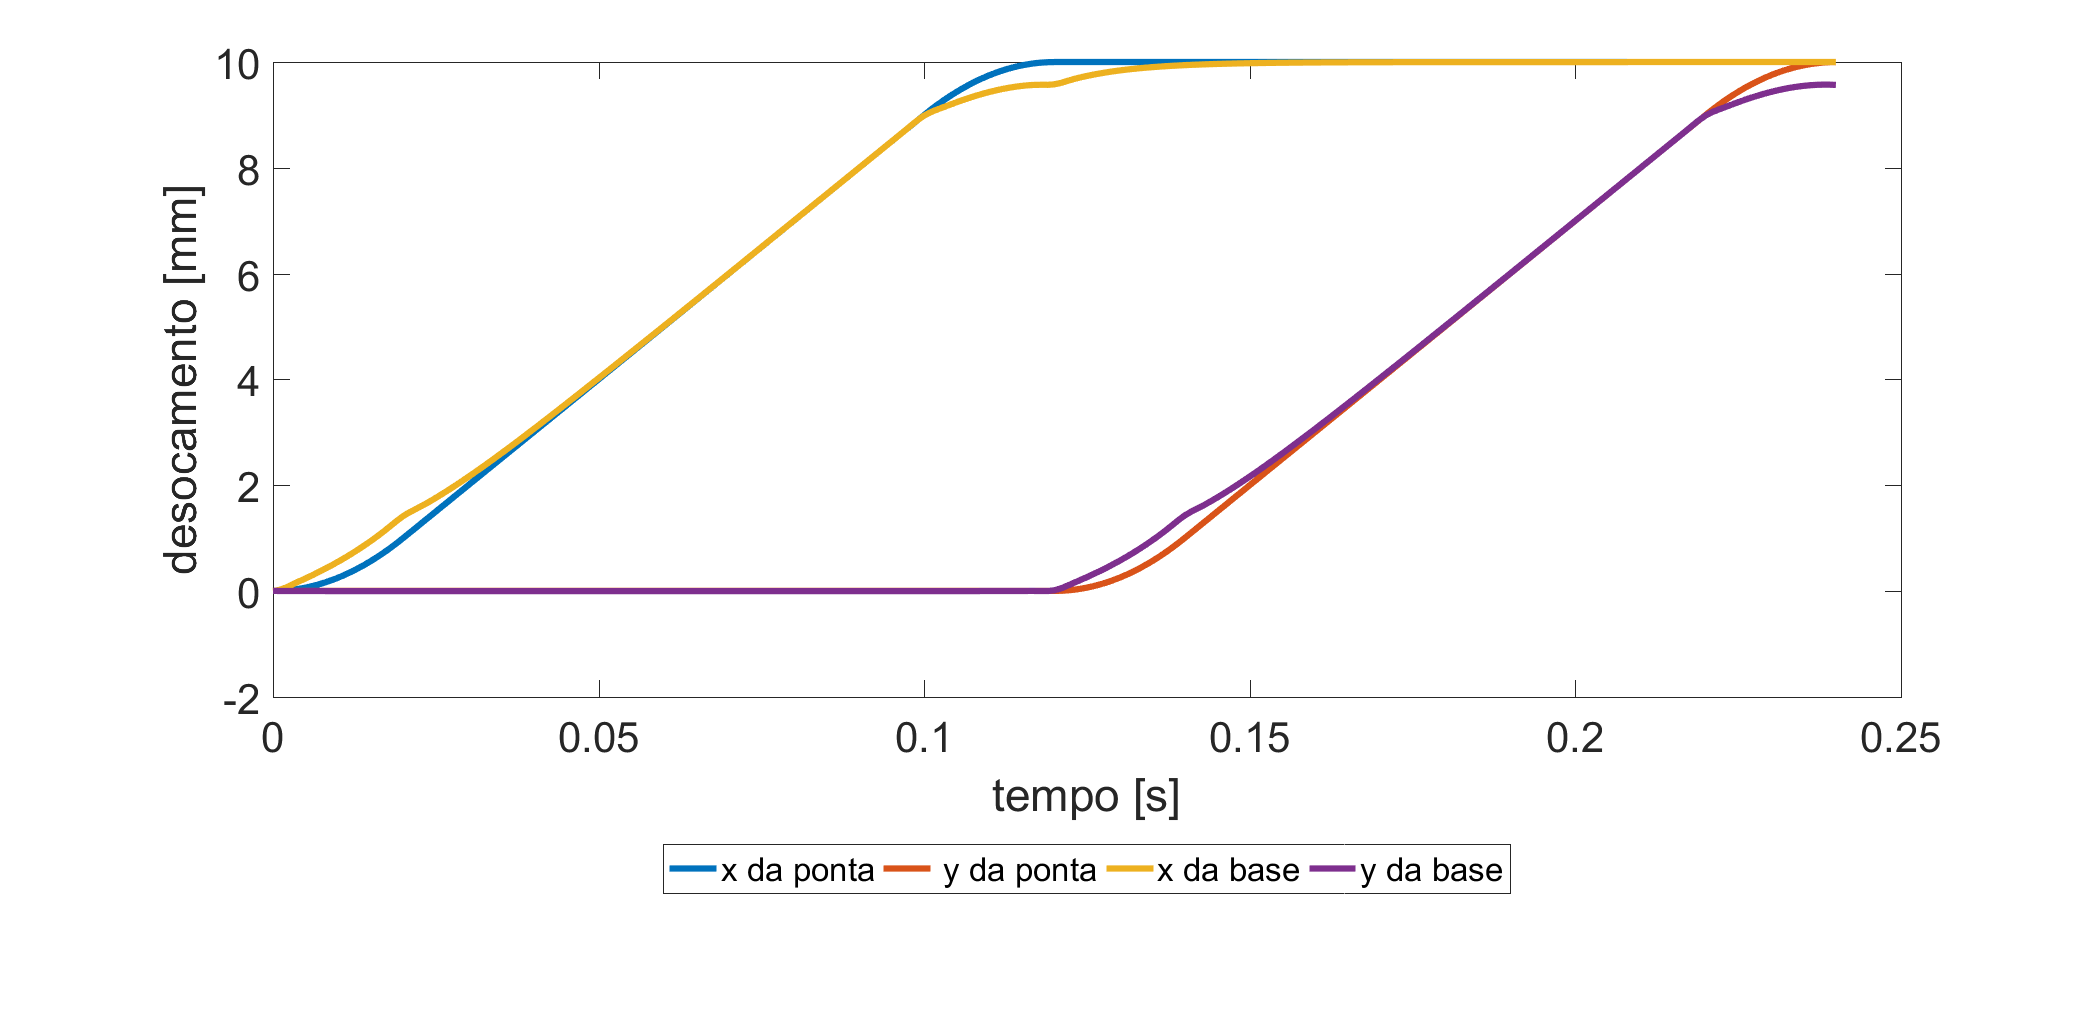
\includegraphics[scale=0.44]{Teste Padrao des}
    \label{fig:t_padr_des}
    \end{center}
\end{figure}    

Trajetória Espacial (Figura \ref{fig:t_padr_pos}): Este gráfico ilustra o caminho percorrido nos planos X e Y, comparando a trajetória da ponta com a trajetória de referência. A aderência ao caminho planejado, conforme descrito na metodologia, é fundamental para avaliar a acurácia do sistema.

\begin{figure}[H]
    \begin{center}
    \caption{Caso referência - Caminho percorrido x vs y da ponta e da referência}
    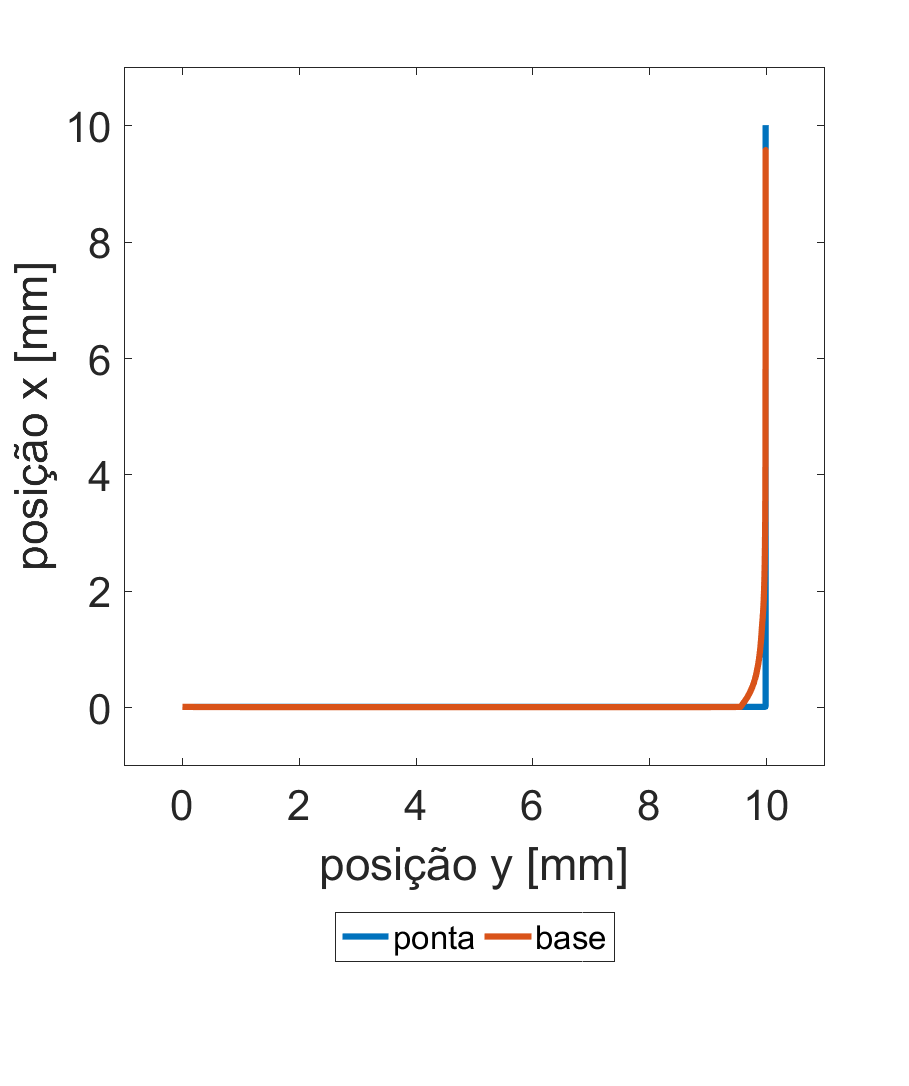
\includegraphics[scale=0.44]{Teste Padrao pos}
    \label{fig:t_padr_pos}
    \end{center}
\end{figure}

O gráfico apresentado na Figura \ref{fig:t_padr_viab} exibe a evolução das iterações durante a simulação. Cada ponto no gráfico representa uma iteração distinta. O eixo X mostra o número de avaliações da função objetivo e das restrições, enquanto o eixo Y reflete o valor de viabilidade, que indica o grau de cumprimento das restrições mais desafiadoras, conforme discutido na metodologia.

Observa-se uma tendência clara de convergência ao longo das iterações, um indicativo de que a simulação está alcançando resultados bem-sucedidos. Notavelmente, os valores iniciais de viabilidade se aproximam de $7,5x10^{-3}$, um padrão consistente observado em vários casos.

Além disso, o tempo total de simulação para esta análise foi de aproximadamente 89,8 segundos. Os vetores de posição empregados na simulação contavam com 241 elementos, refletindo a complexidade e a precisão dos cálculos realizados.

Este gráfico é fundamental para entender a eficácia da simulação em atender às restrições estabelecidas e a capacidade do sistema de convergir para uma solução viável em um tempo eficiente.

\begin{figure}[H]
    \begin{center}
    \caption{Caso referência - Num de fun x Viabilidade}
    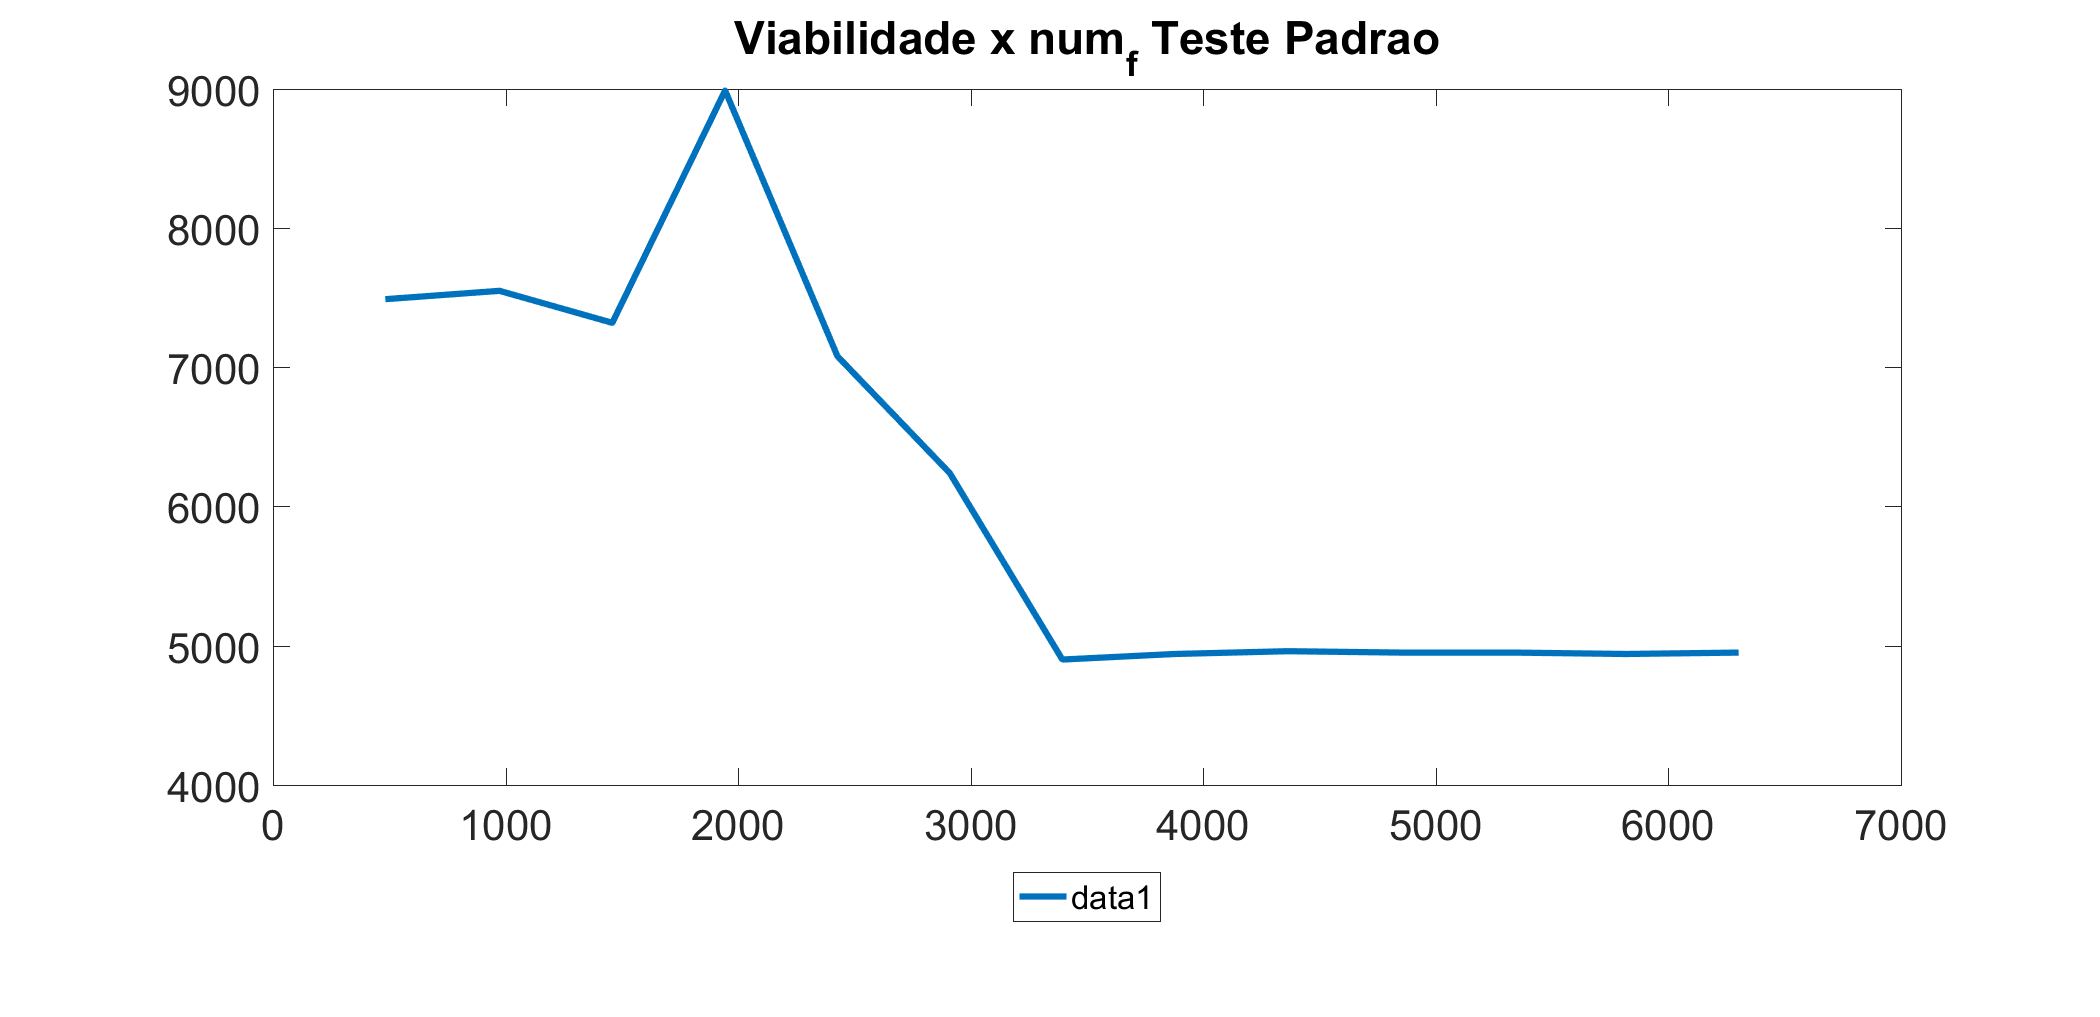
\includegraphics[scale=0.44]{Teste Padrao Viabilidade}
    \label{fig:t_padr_viab}
    \end{center}
\end{figure}

\section{Análise de Sensibilidade dos Resultados}
\subsection{Caso 1 - Variação da frequência}
Este caso investiga como a variação da frequência natural afeta o modelo dinâmico do sistema. A frequência natural, sendo um parâmetro crítico, influencia diretamente o comportamento da planta do modelo, com implicações notáveis nas amplitudes dos desvios e na necessidade de compensação.

Observamos que sistemas com maior rigidez, caracterizados por frequências naturais mais altas, exibem menores amplitudes de desvio e uma reduzida necessidade de compensação. Esta tendência é claramente ilustrada ao comparar as figuras \ref{fig:t_1a_vels}, \ref{fig:t_1b_vels} e \ref{fig:t_1c_vels}, que mostram o comportamento das velocidades em x e y para diferentes configurações de frequência.

\begin{figure}[H]
    \begin{center}
    \caption{Caso 1A - Comportamento no tempo das velocidades em x e y da ponta e da referência}
    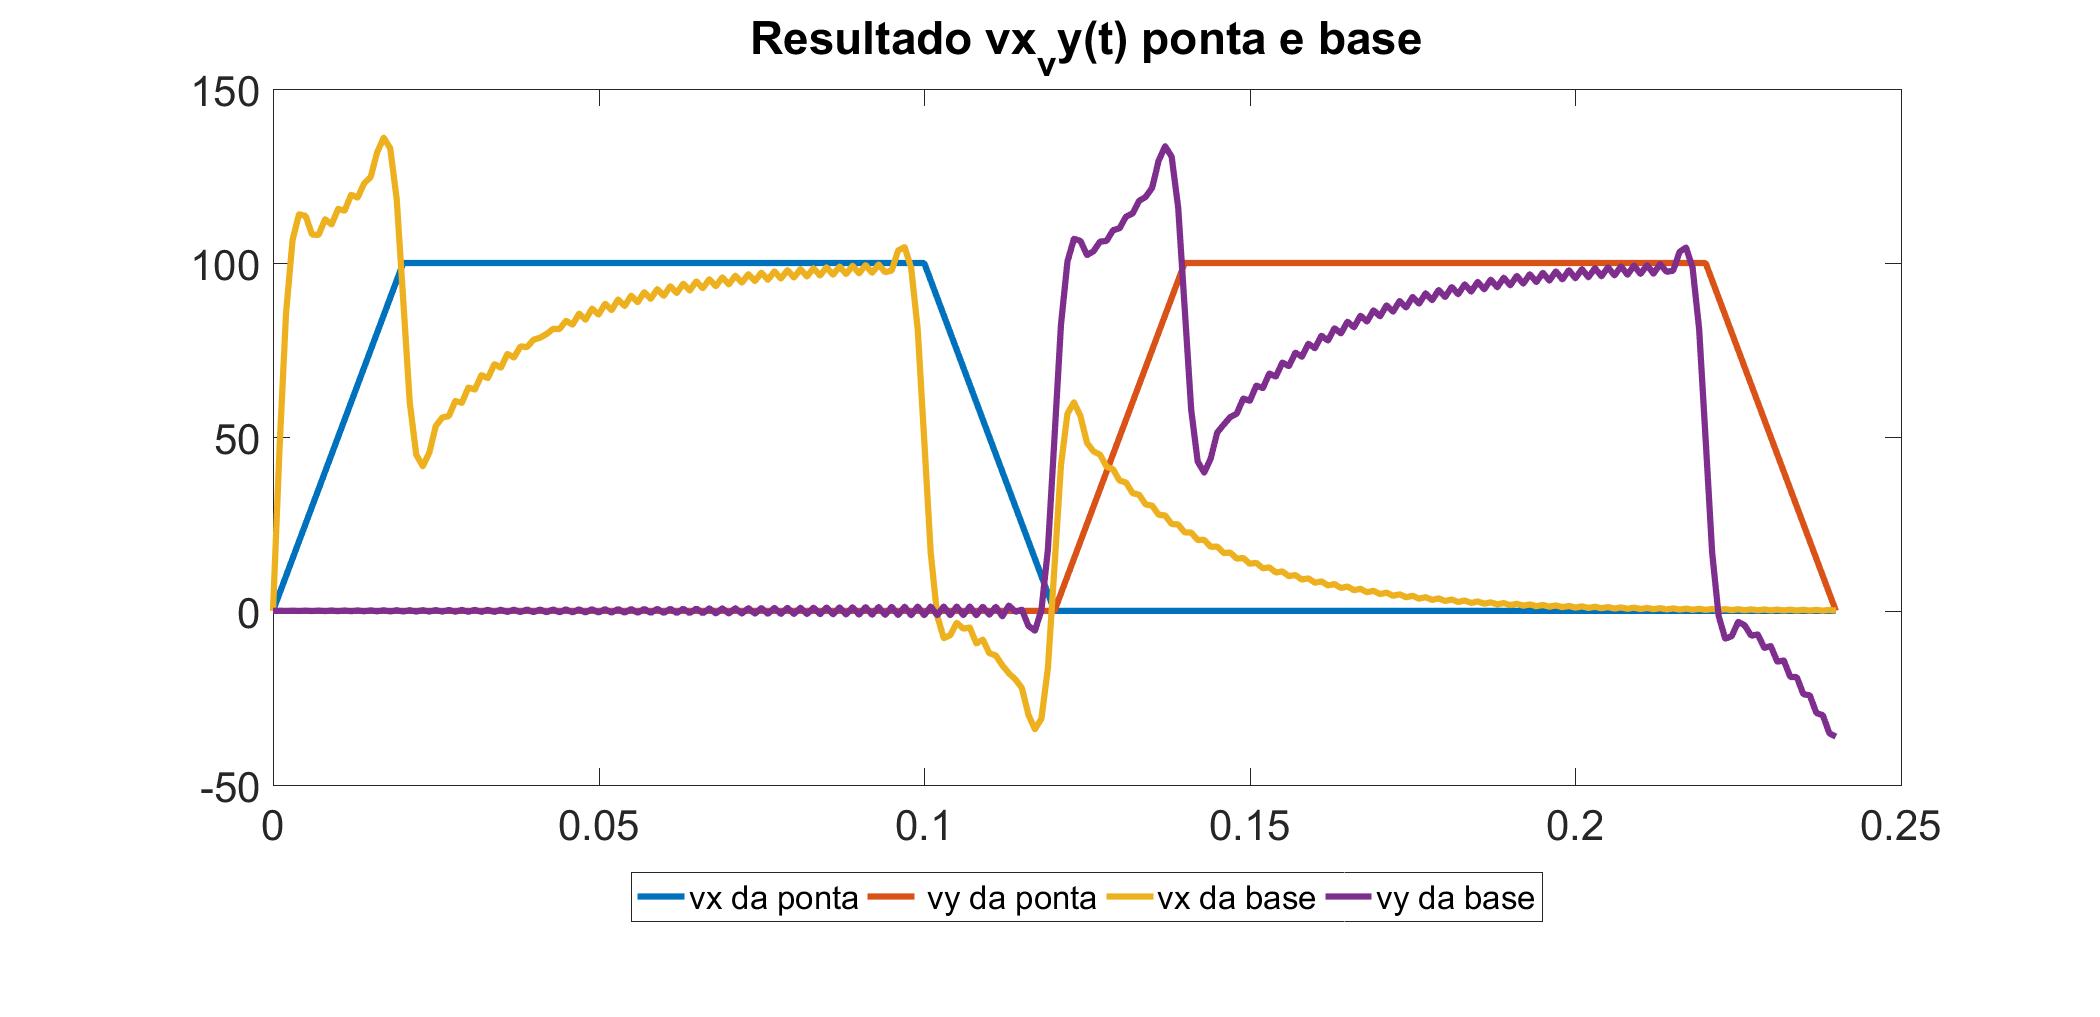
\includegraphics[scale=0.44]{Teste 1 A vels}
    \label{fig:t_1a_vels}
    \end{center}
\end{figure}

\begin{figure}[H]
    \begin{center}
    \caption{Caso 1B - Comportamento no tempo das velocidades em x e y da ponta e da referência}
    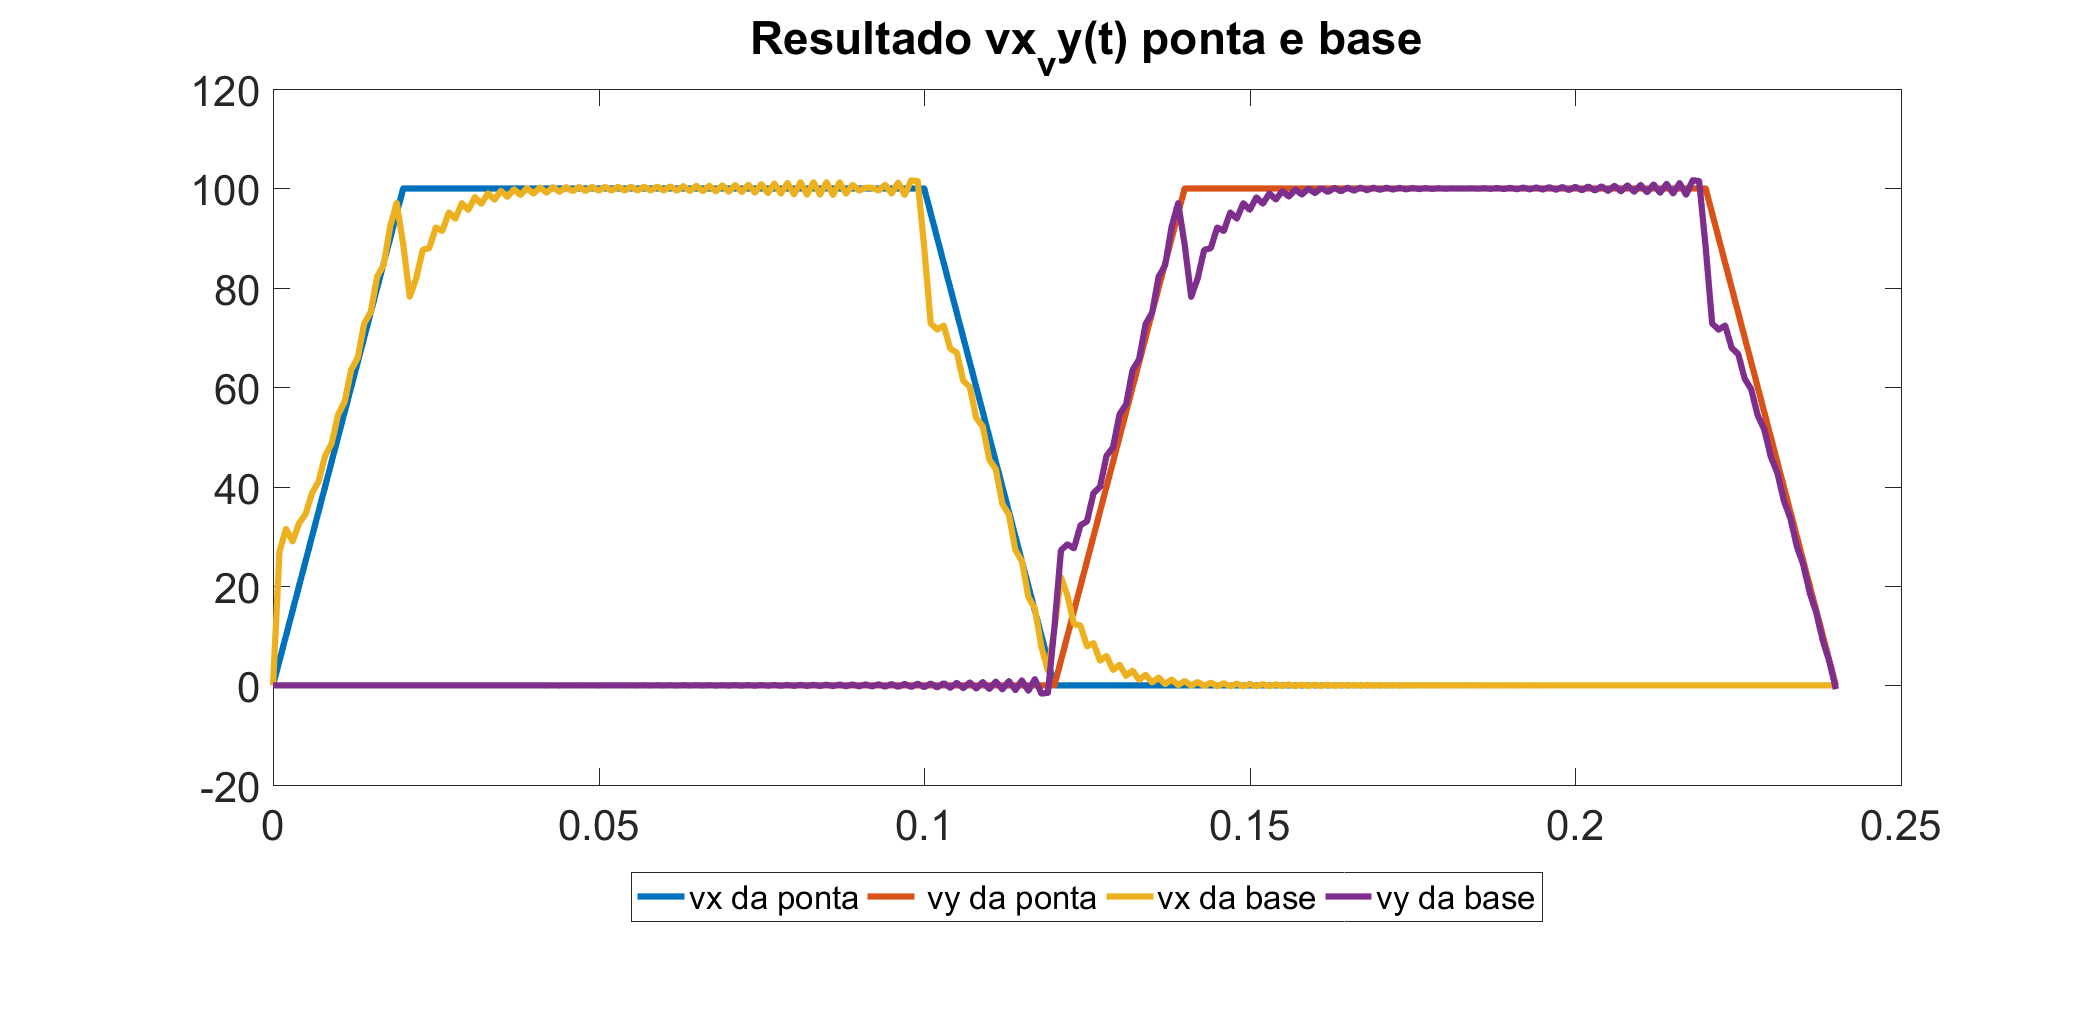
\includegraphics[scale=0.44]{Teste 1 B vels}
    \label{fig:t_1b_vels}
    \end{center}
\end{figure}

\begin{figure}[H]
    \begin{center}
    \caption{Caso 1C - Comportamento no tempo das velocidades em x e y da ponta e da referência}
    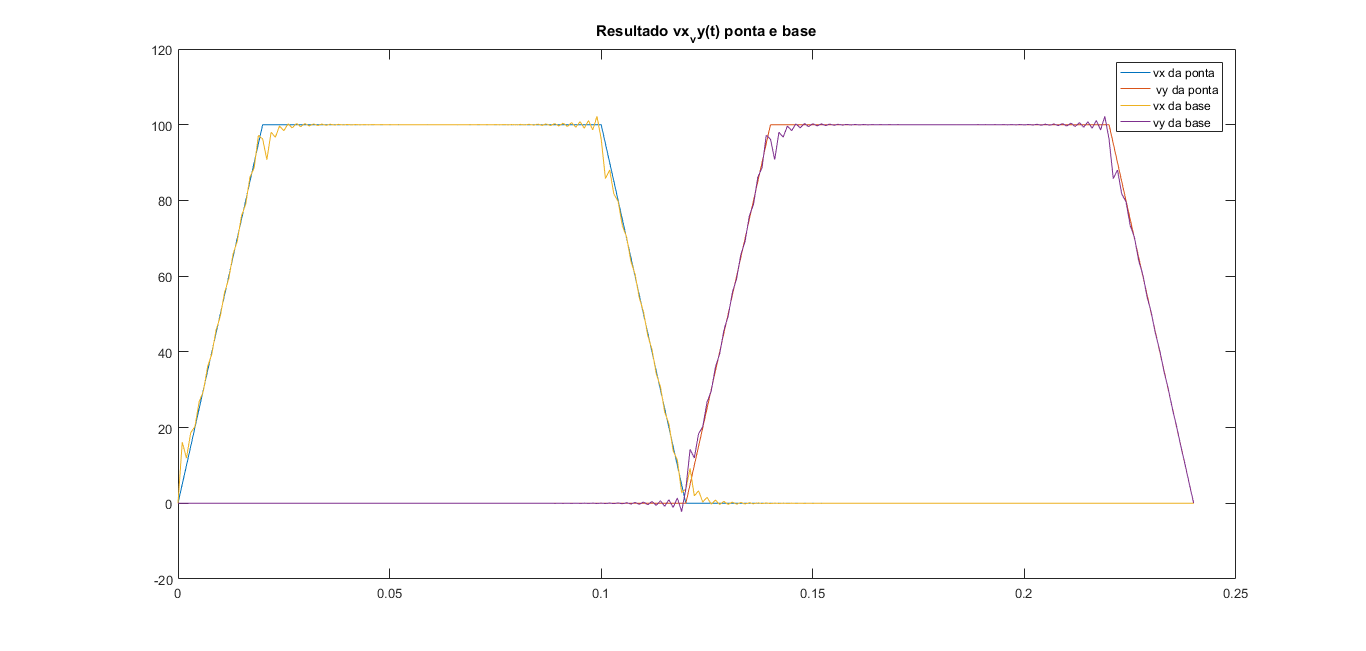
\includegraphics[scale=0.44]{Teste 1 C vels}
    \label{fig:t_1c_vels}
    \end{center}
\end{figure}

A análise é aprofundada ao examinar as figuras \ref{fig:t_1a_des}, \ref{fig:t_1c_des}, \ref{fig:t_1a_pos} e \ref{fig:t_1c_pos}, que revelam as diferenças no comportamento do deslocamento e no caminho percorrido pela ponta do sistema nos extremos do caso (A e C). Estes resultados indicam que variações na frequência natural não apenas afetam as propriedades dinâmicas, mas também têm implicações diretas no controle e precisão do sistema.

\begin{figure}[H]
    \begin{center}
    \caption{Caso 1A - Comportamento no tempo dos deslocamentos em x e y da ponta e da referência}
    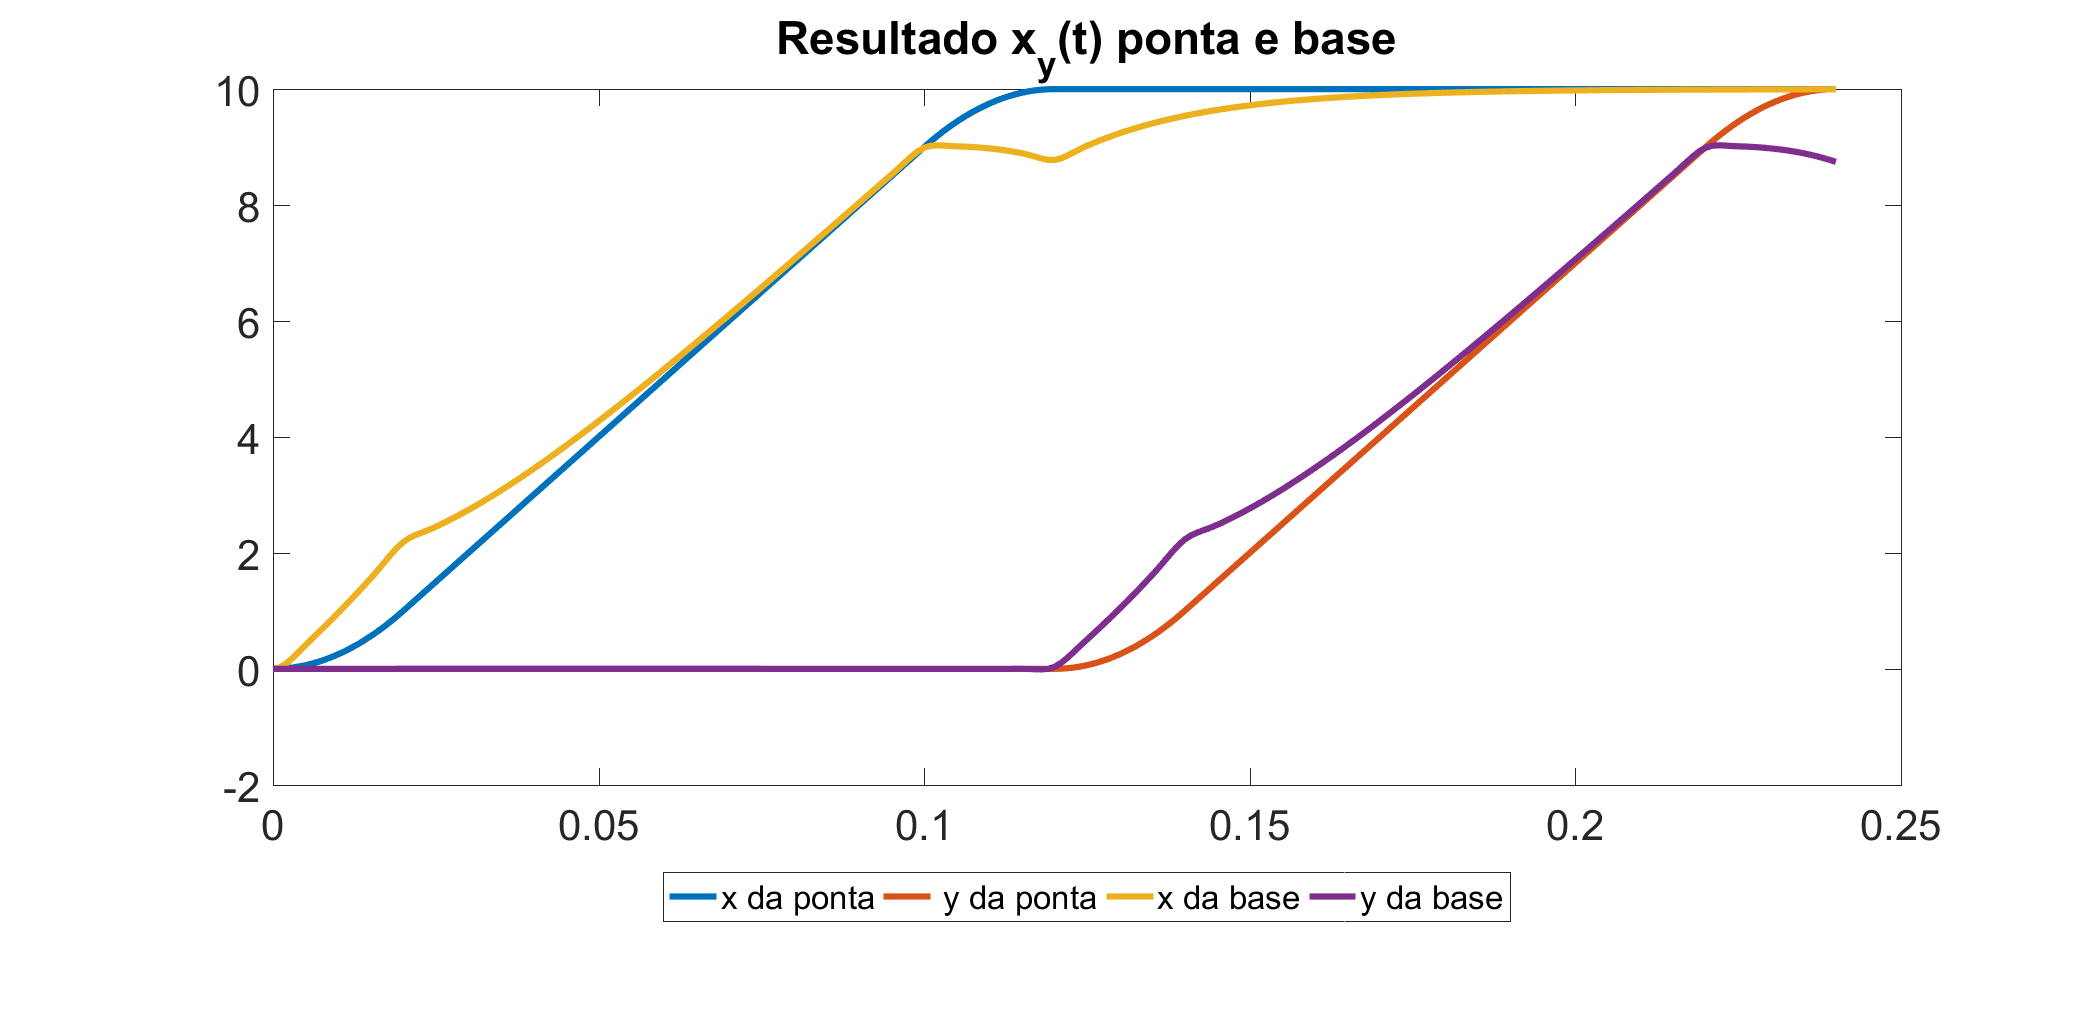
\includegraphics[scale=0.44]{Teste 1 A des}
    \label{fig:t_1a_des}
    \end{center}
\end{figure}

\begin{figure}[H]
    \begin{center}
    \caption{Caso 1C - Comportamento no tempo dos deslocamentos em x e y da ponta e da referência}
    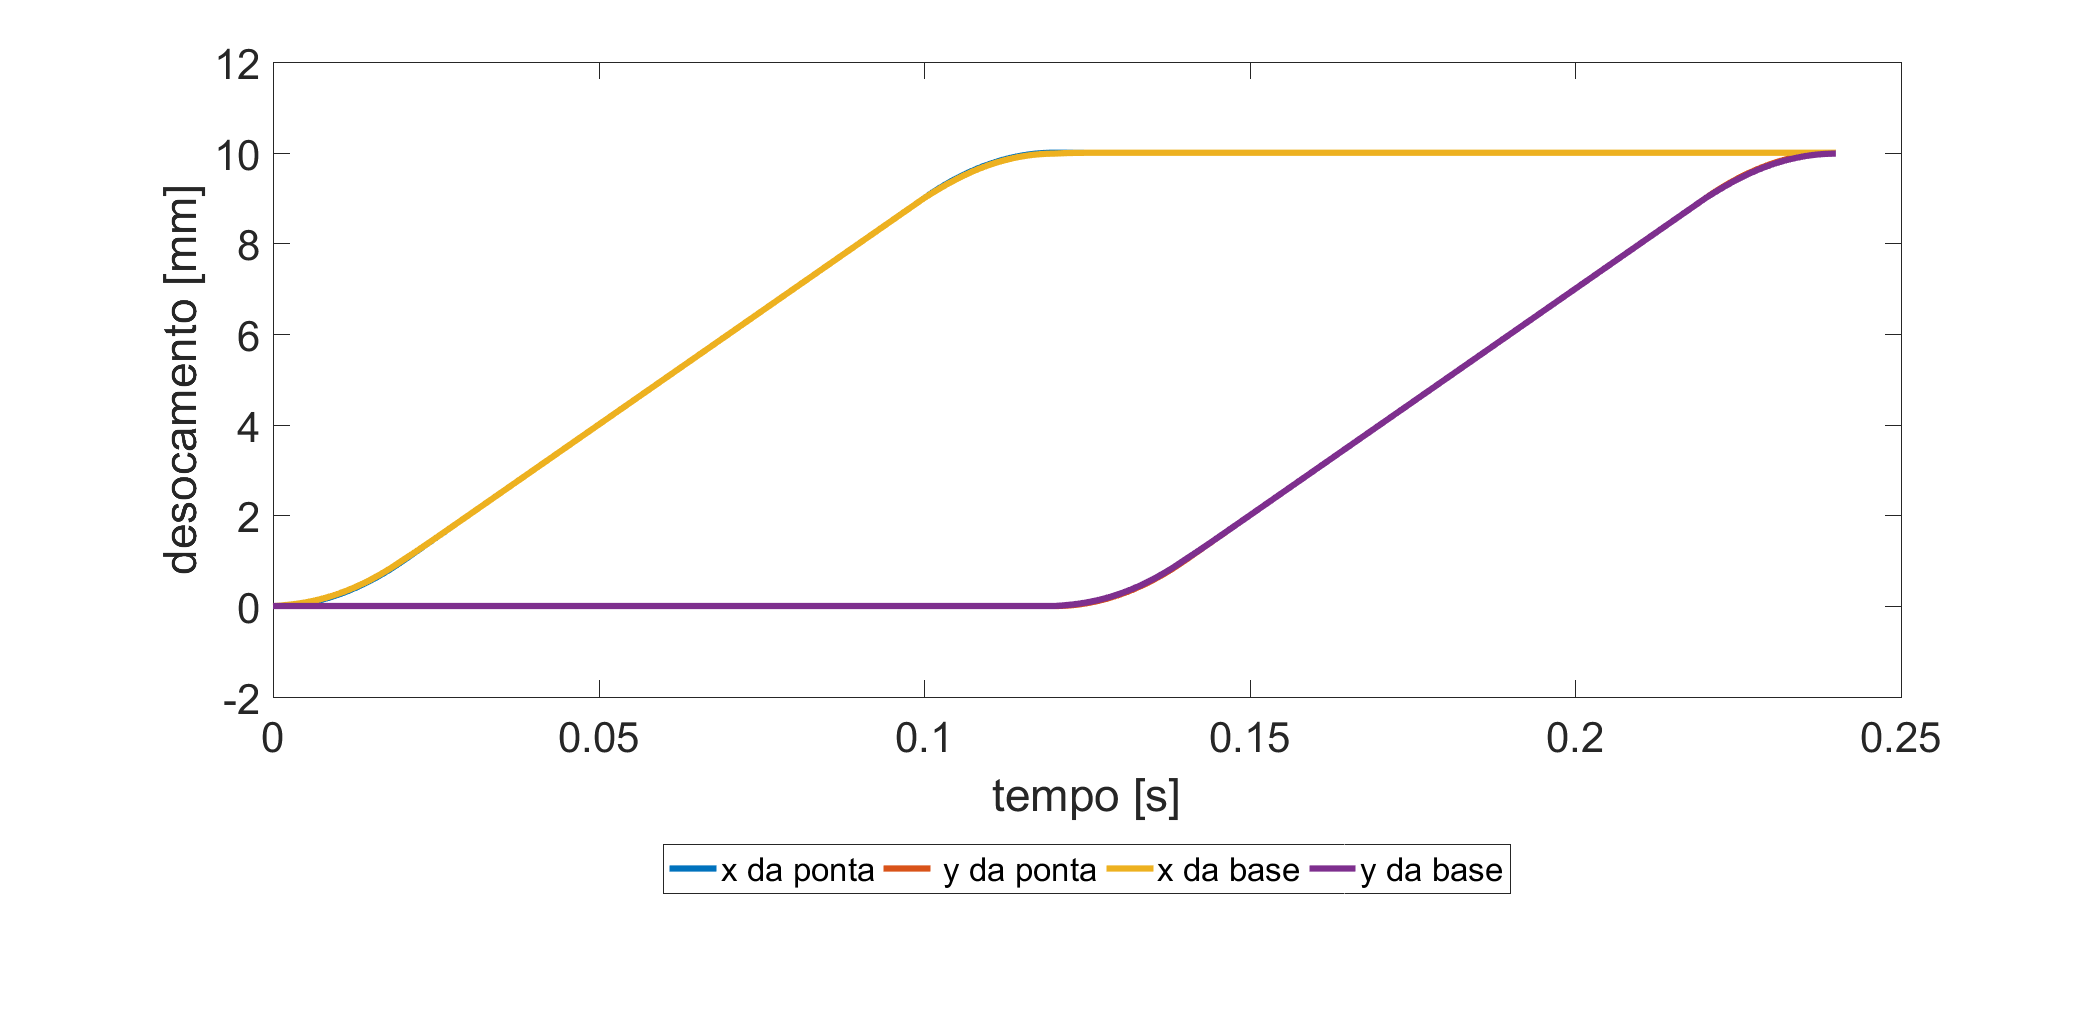
\includegraphics[scale=0.44]{Teste 1 C des}
    \label{fig:t_1c_des}
    \end{center}
\end{figure}

\begin{figure}[H]
    \begin{center}
    \caption{Caso 1A - Caminho percorrido x vs y da ponta e da referência}
    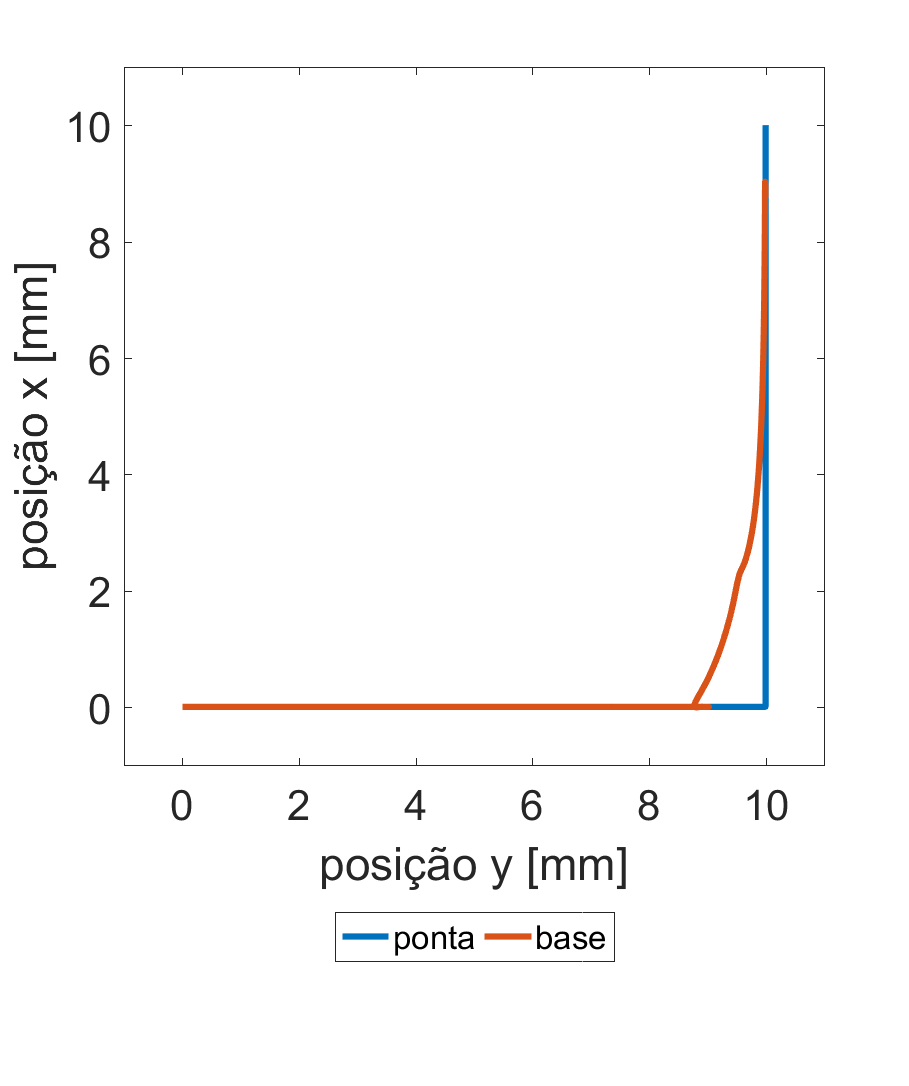
\includegraphics[scale=0.44]{Teste 1 A pos}
    \label{fig:t_1a_pos}
    \end{center}
\end{figure}

\begin{figure}[H]
    \begin{center}
    \caption{Caso 1C - Caminho percorrido x vs y da ponta e da referência}
    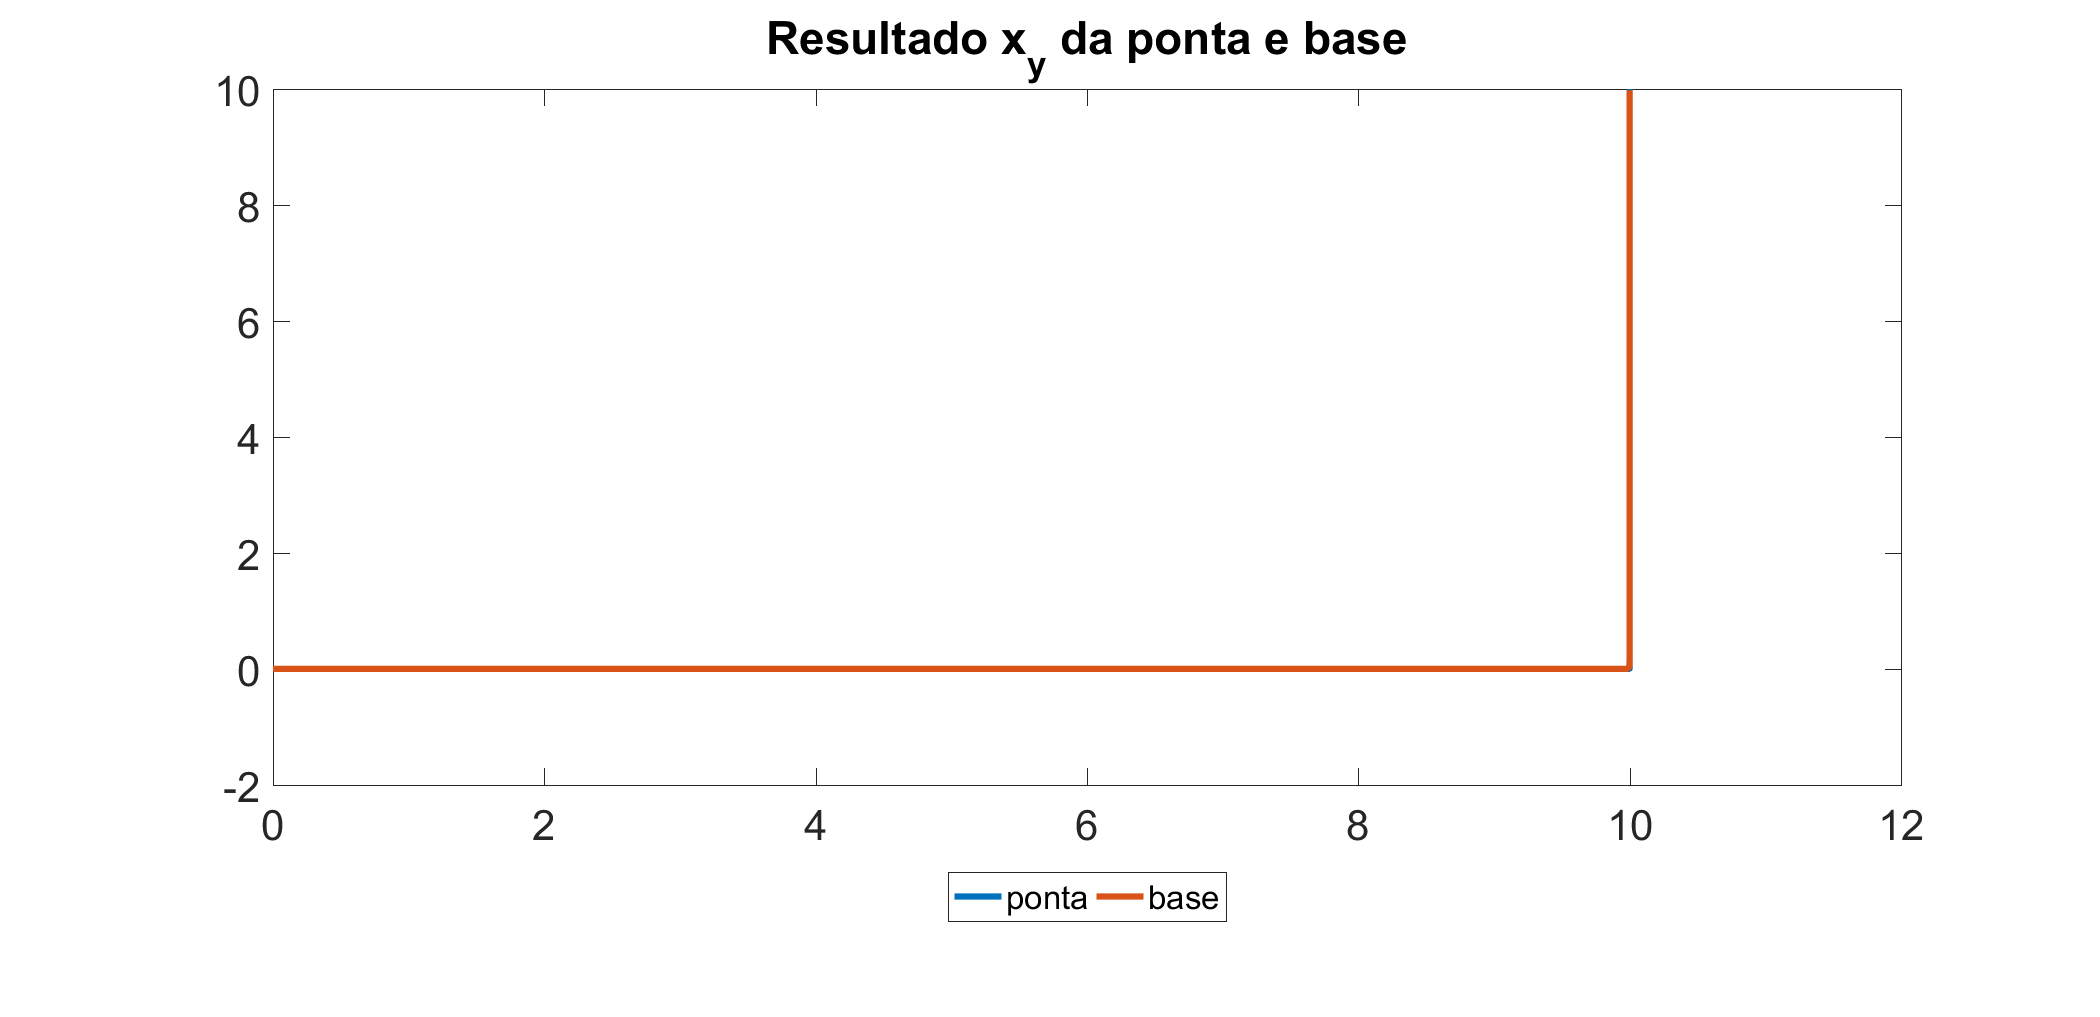
\includegraphics[scale=0.44]{Teste 1 C pos}
    \label{fig:t_1c_pos}
    \end{center}
\end{figure}

Além disso, a figura \ref{fig:t_1_viab} fornece uma visão geral da viabilidade do sistema sob diferentes configurações de frequência natural. Observamos um padrão de convergência similar em todos os casos, mas com uma viabilidade menor e, consequentemente, menores violações das restrições impostas nos casos de maior rigidez. Isso reflete um equilíbrio mais eficiente entre precisão e esforço computacional.

\begin{figure}[H]
    \begin{center}
    \caption{Caso 1 - Num de fun x Viabilidade}
    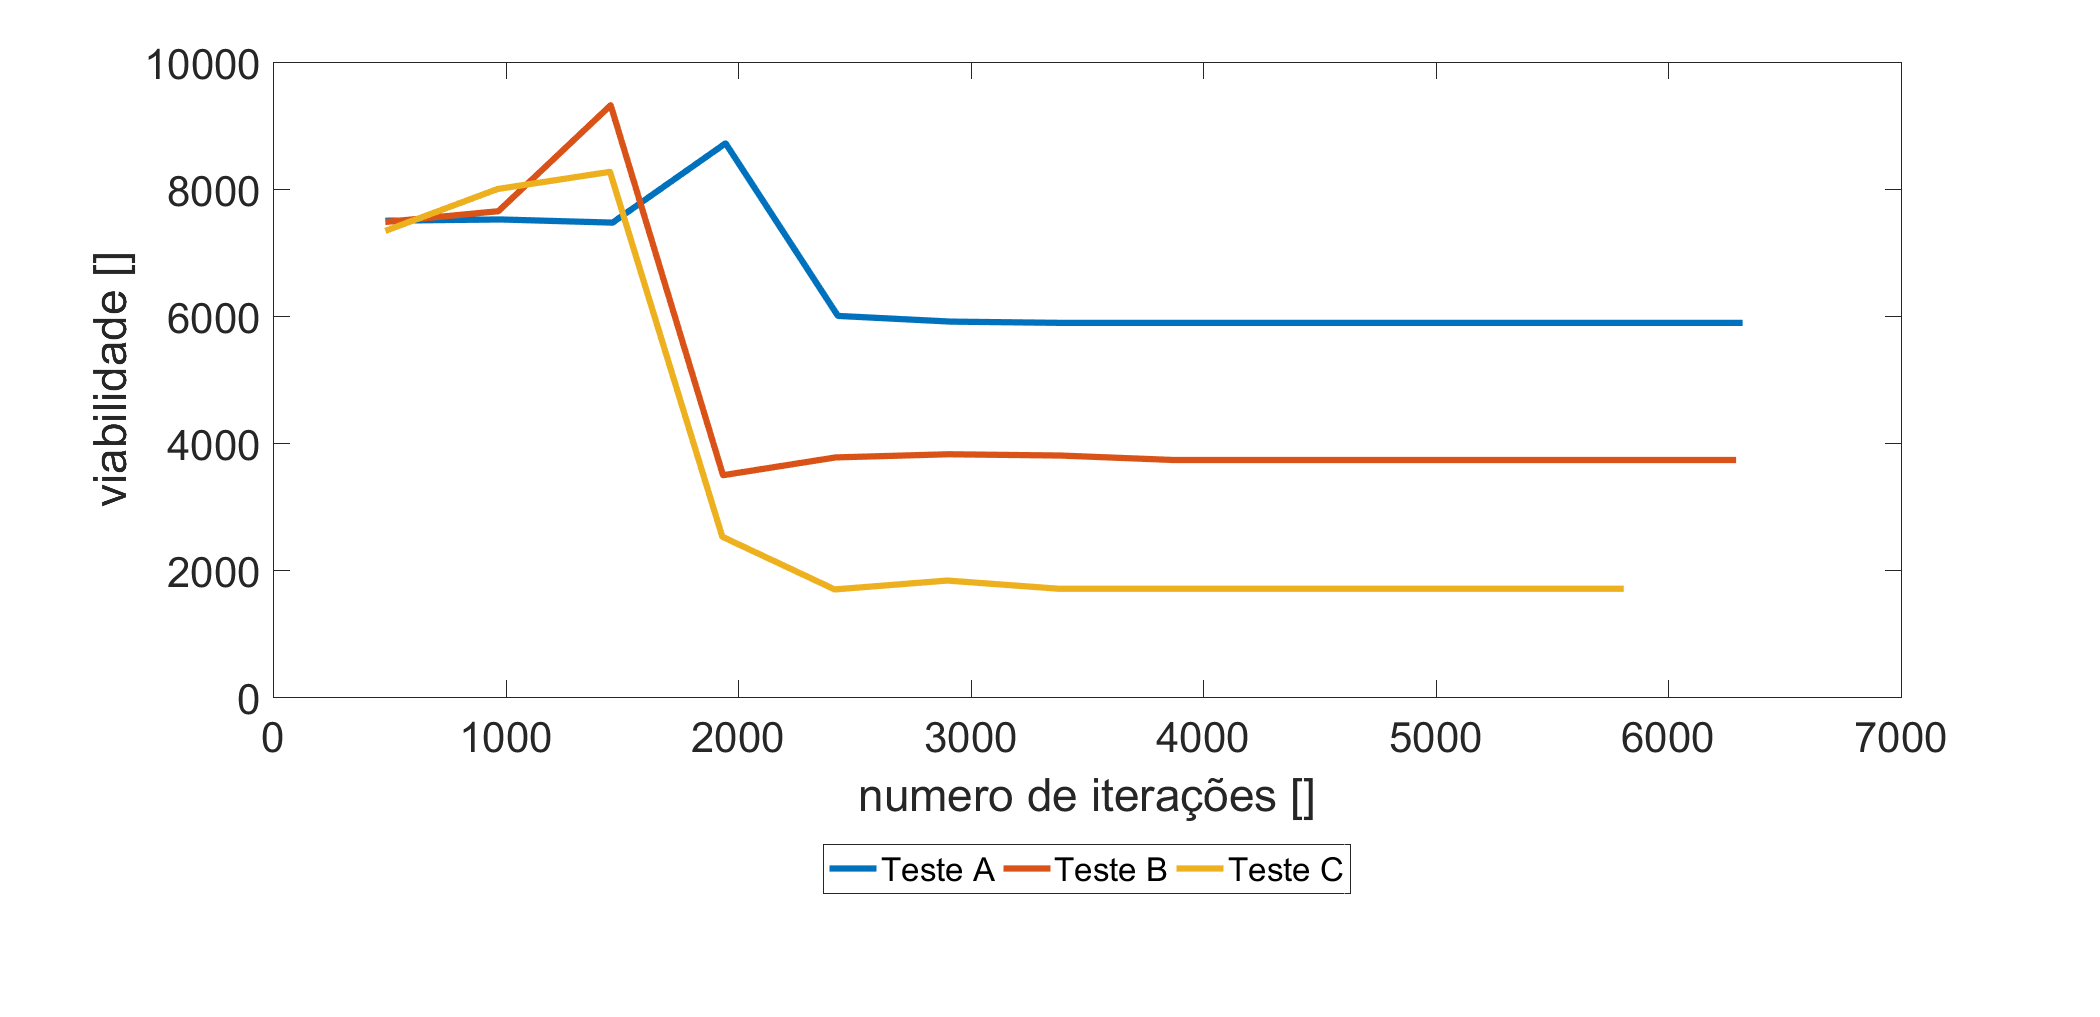
\includegraphics[scale=0.44]{Teste 1 Viabilidade}
    \label{fig:t_1_viab}
    \end{center}
\end{figure}

Importante também é o impacto dessas variações na frequência natural no tempo de simulação. Observamos que os tempos de simulação variaram de 96,76 segundos no Caso A até 80,77 segundos no Caso C, com o Caso B intermediário, em 89,04 segundos. Esta tendência sugere que sistemas com maior rigidez (frequências naturais mais altas) não apenas melhoram a eficácia em termos de cumprimento das restrições, mas também podem levar a uma simulação mais rápida, apesar de todos os casos utilizarem vetores de posição com 241 elementos. Esta observação é crítica para aplicações práticas, onde a eficiência computacional e a rapidez na resposta são essenciais.

\subsection{Caso 2 - Variação do coeficiente de amortecimento}
Neste caso, investigamos o impacto de diferentes coeficientes de amortecimento no comportamento do sistema. As Figuras \ref{fig:t_2b_pos} e \ref{fig:t_2c_pos} são cruciais para esta análise, pois ilustram as trajetórias espaciais para as variações B e C do coeficiente de amortecimento. Estes resultados são contrastados com a Figura \ref{fig:t_padr_pos}, que representa um coeficiente intermediário, oferecendo uma comparação direta entre os extremos e o caso base.

\begin{figure}[H]
    \begin{center}
    \caption{Caso 2B - Caminho percorrido x vs y da ponta e da referência}
    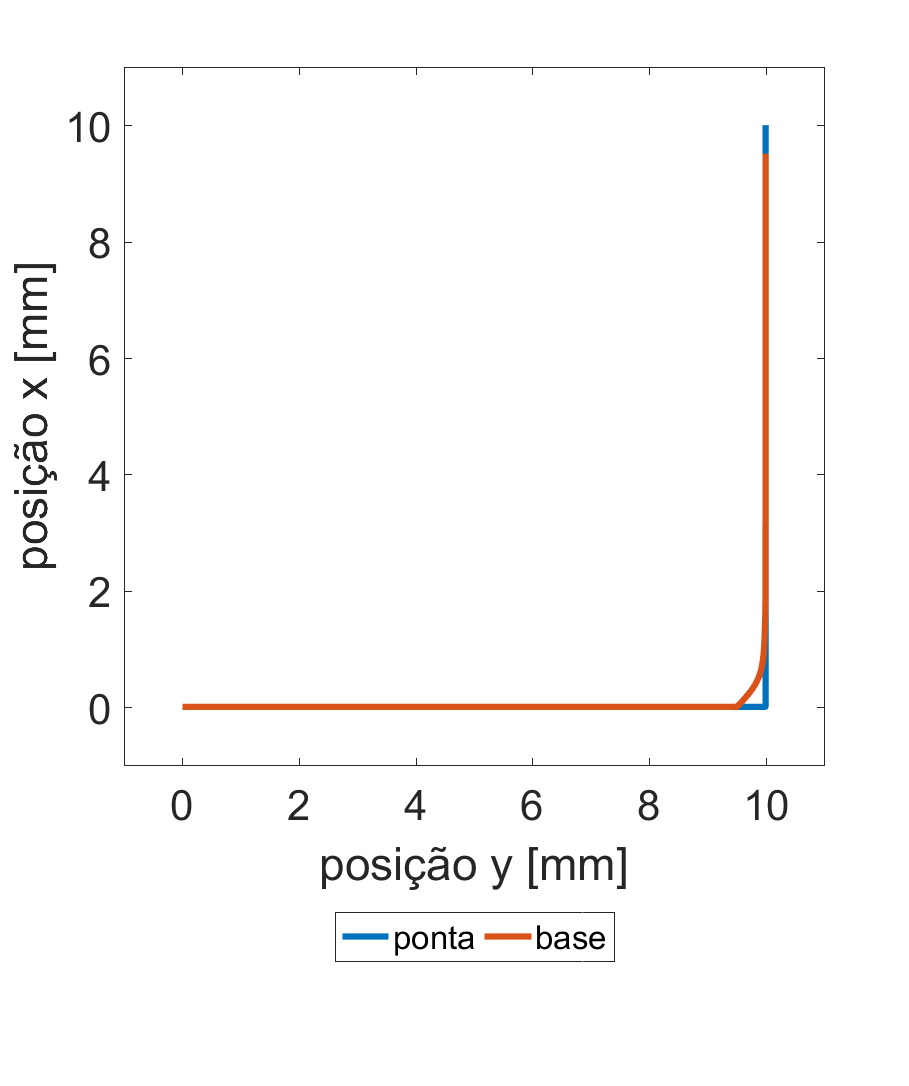
\includegraphics[scale=0.44]{Teste 2 B pos}
    \label{fig:t_2b_pos}
    \end{center}
\end{figure}

\begin{figure}[H]
    \begin{center}
    \caption{Caso 2C - Caminho percorrido x vs y da ponta e da referência}
    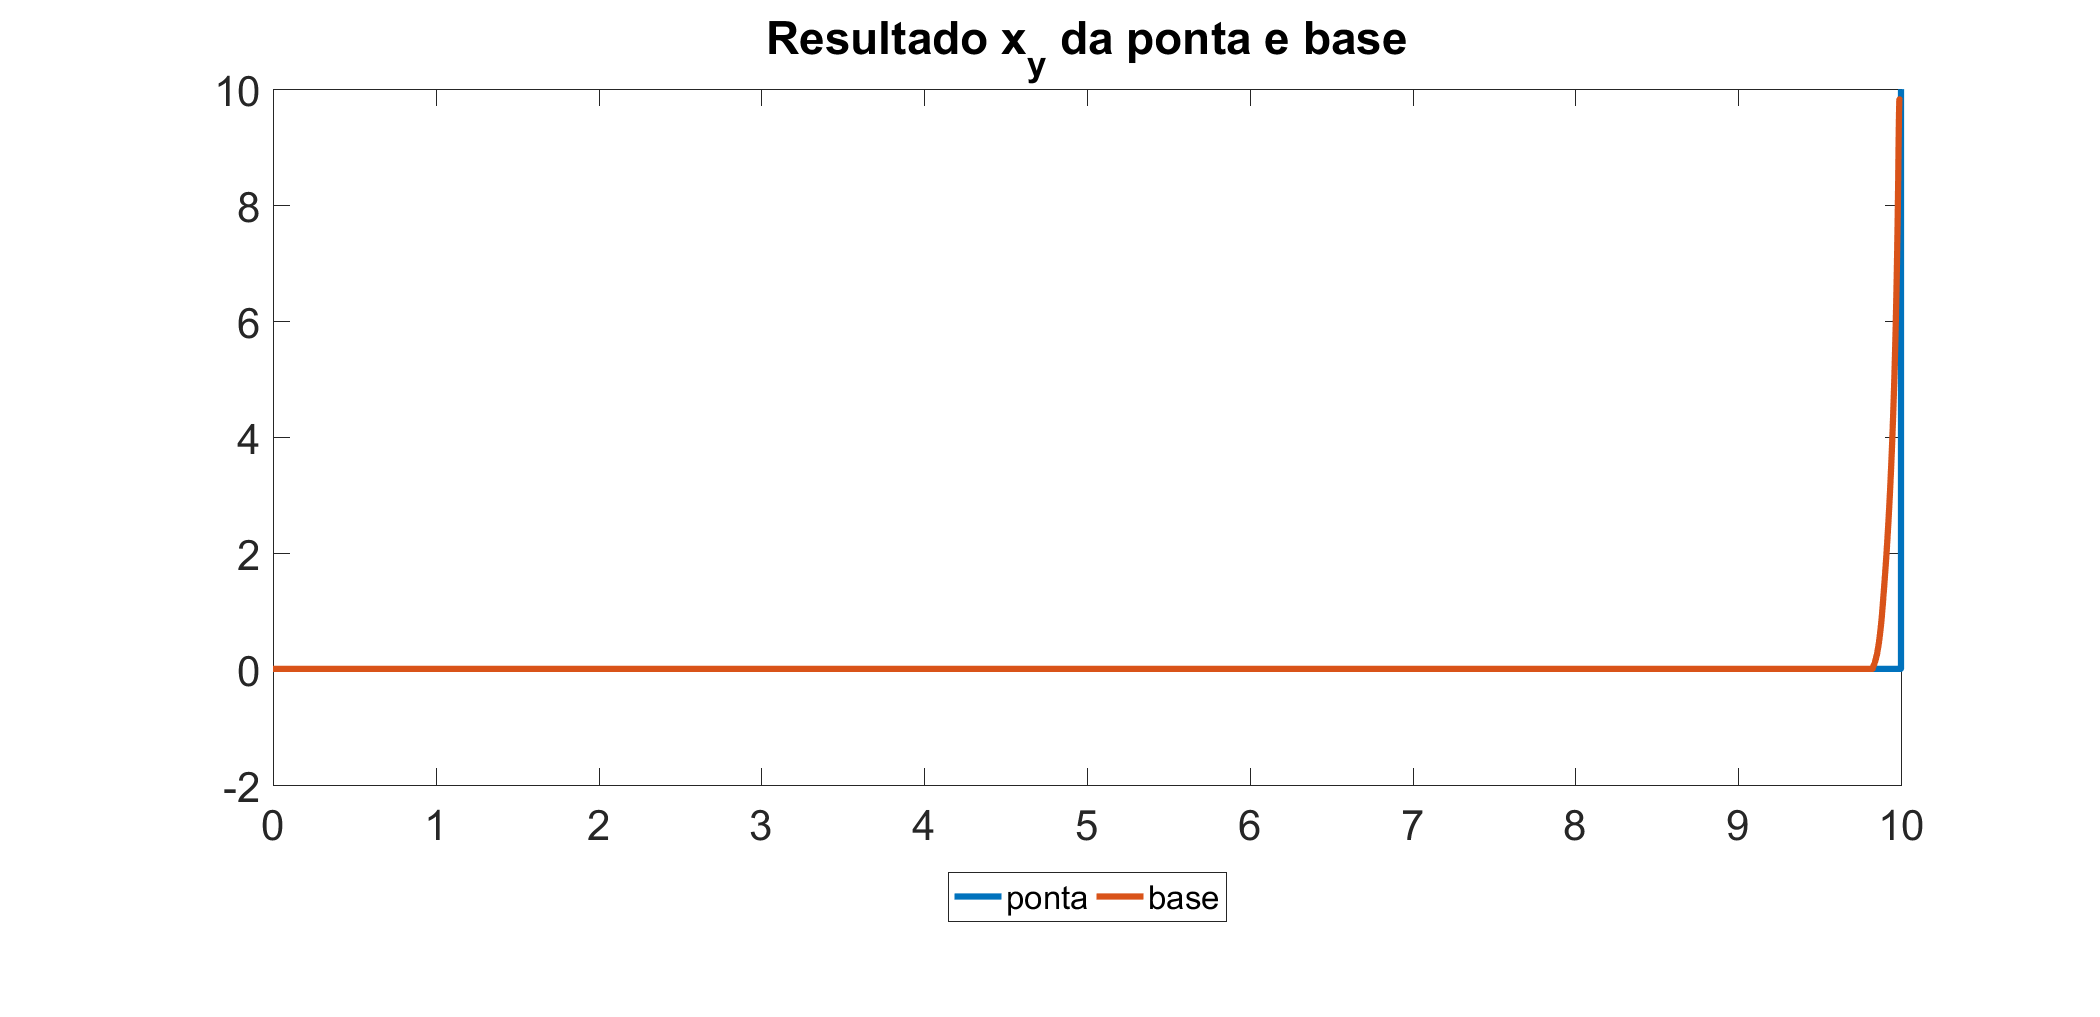
\includegraphics[scale=0.44]{Teste 2 C pos}
    \label{fig:t_2c_pos}
    \end{center}
\end{figure}

Curiosamente, o Caso A, que não conseguiu convergir e apresentou valores de entrada similares aos outros casos, serve como um exemplo notável de como variações no coeficiente de amortecimento podem levar a comportamentos divergentes. Este fenômeno é evidenciado na figura \ref{fig:t_2_viab}, onde observamos uma tendência de convergência para valores de viabilidade menores à medida que o coeficiente de amortecimento aumenta. Isso sugere uma maior facilidade em compensar desvios quando o coeficiente é elevado.

\begin{figure}[H]
    \begin{center}
    \caption{Caso 2 - Num de fun x Viabilidade}
    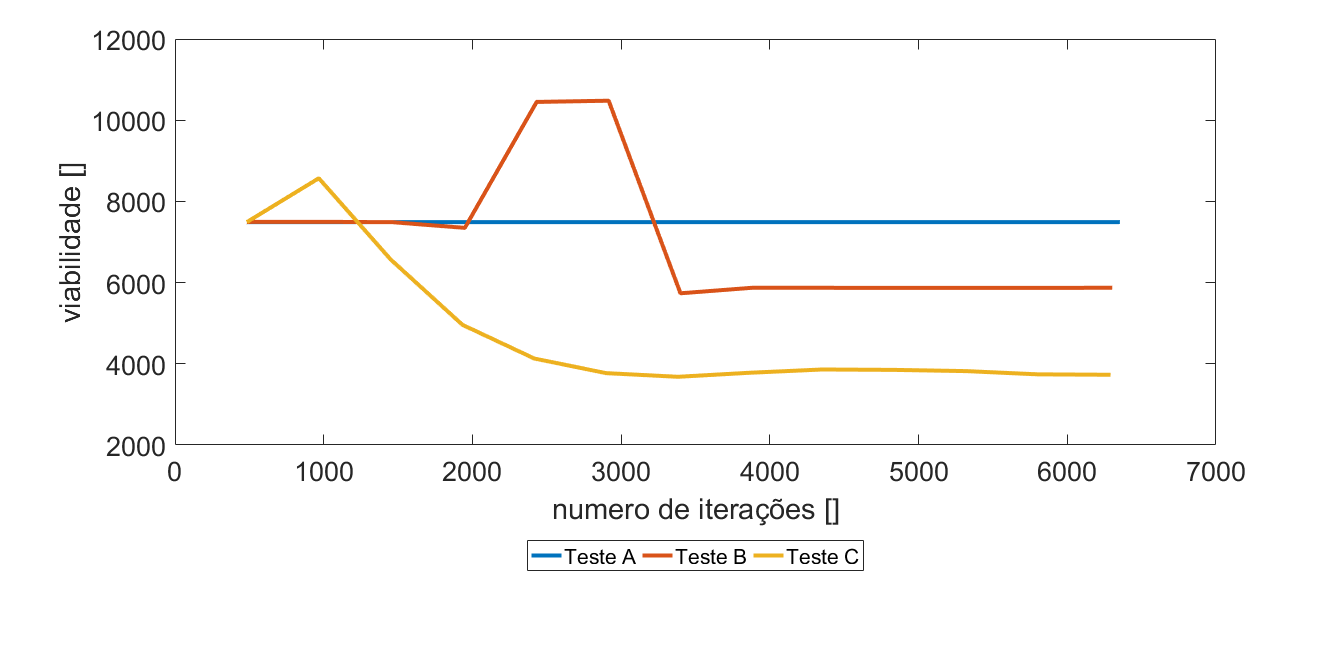
\includegraphics[scale=0.44]{Teste 2 Viabilidade}
    \label{fig:t_2_viab}
    \end{center}
\end{figure}

Em termos de desempenho computacional, todos os casos mantiveram uma consistência, com 241 elementos nos vetores de posição. Os tempos de simulação foram de 69, 89 e 52 segundos para os Casos 2A, 2B e 2C, respectivamente. Estes resultados indicam que, apesar das variações no coeficiente de amortecimento, a simulação manteve uma eficiência computacional comparável entre os diferentes casos.

\subsection{Caso 3 - Variação na aceleração}
Neste caso, focamos na influência da variação da aceleração na geração de comandos do sistema. A figura \ref{fig:t_3a_vels} é central nesta análise, pois ela revela uma forma distinta na curva de velocidade. Com a redução da aceleração, a velocidade não atingiu o patamar desejado, resultando em uma curva com formato triangular. Este comportamento destaca a sensibilidade do sistema às mudanças na aceleração e como isso afeta a capacidade de atingir velocidades alvo.

\begin{figure}[H]
    \begin{center}
    \caption{Caso 3A - Comportamento no tempo das velocidades em x e y da ponta e da referência}
    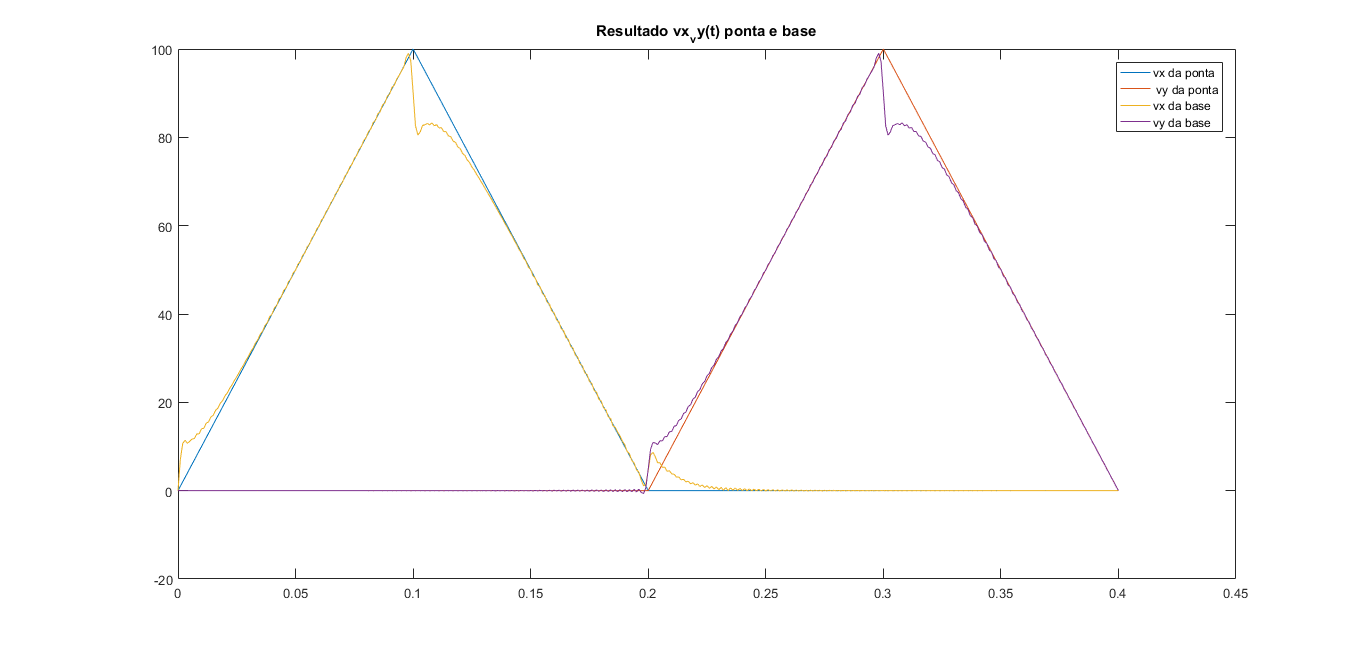
\includegraphics[scale=0.44]{Teste 3 A vels}
    \label{fig:t_3a_vels}
    \end{center}
\end{figure}

A figura \ref{fig:t_3_viab} fornece uma visão adicional sobre as dificuldades encontradas no Caso A. Ao contrário do Caso B, que mostrou um padrão de resposta semelhante aos casos anteriores, o Caso A enfrentou desafios significativos, como evidenciado por um aumento nos valores de viabilidade. Esta discrepância sugere que as variações na aceleração têm um impacto considerável na capacidade do sistema de satisfazer as restrições impostas.

\begin{figure}[H]
    \begin{center}
    \caption{Caso 3 - Num de fun x Viabilidade}
    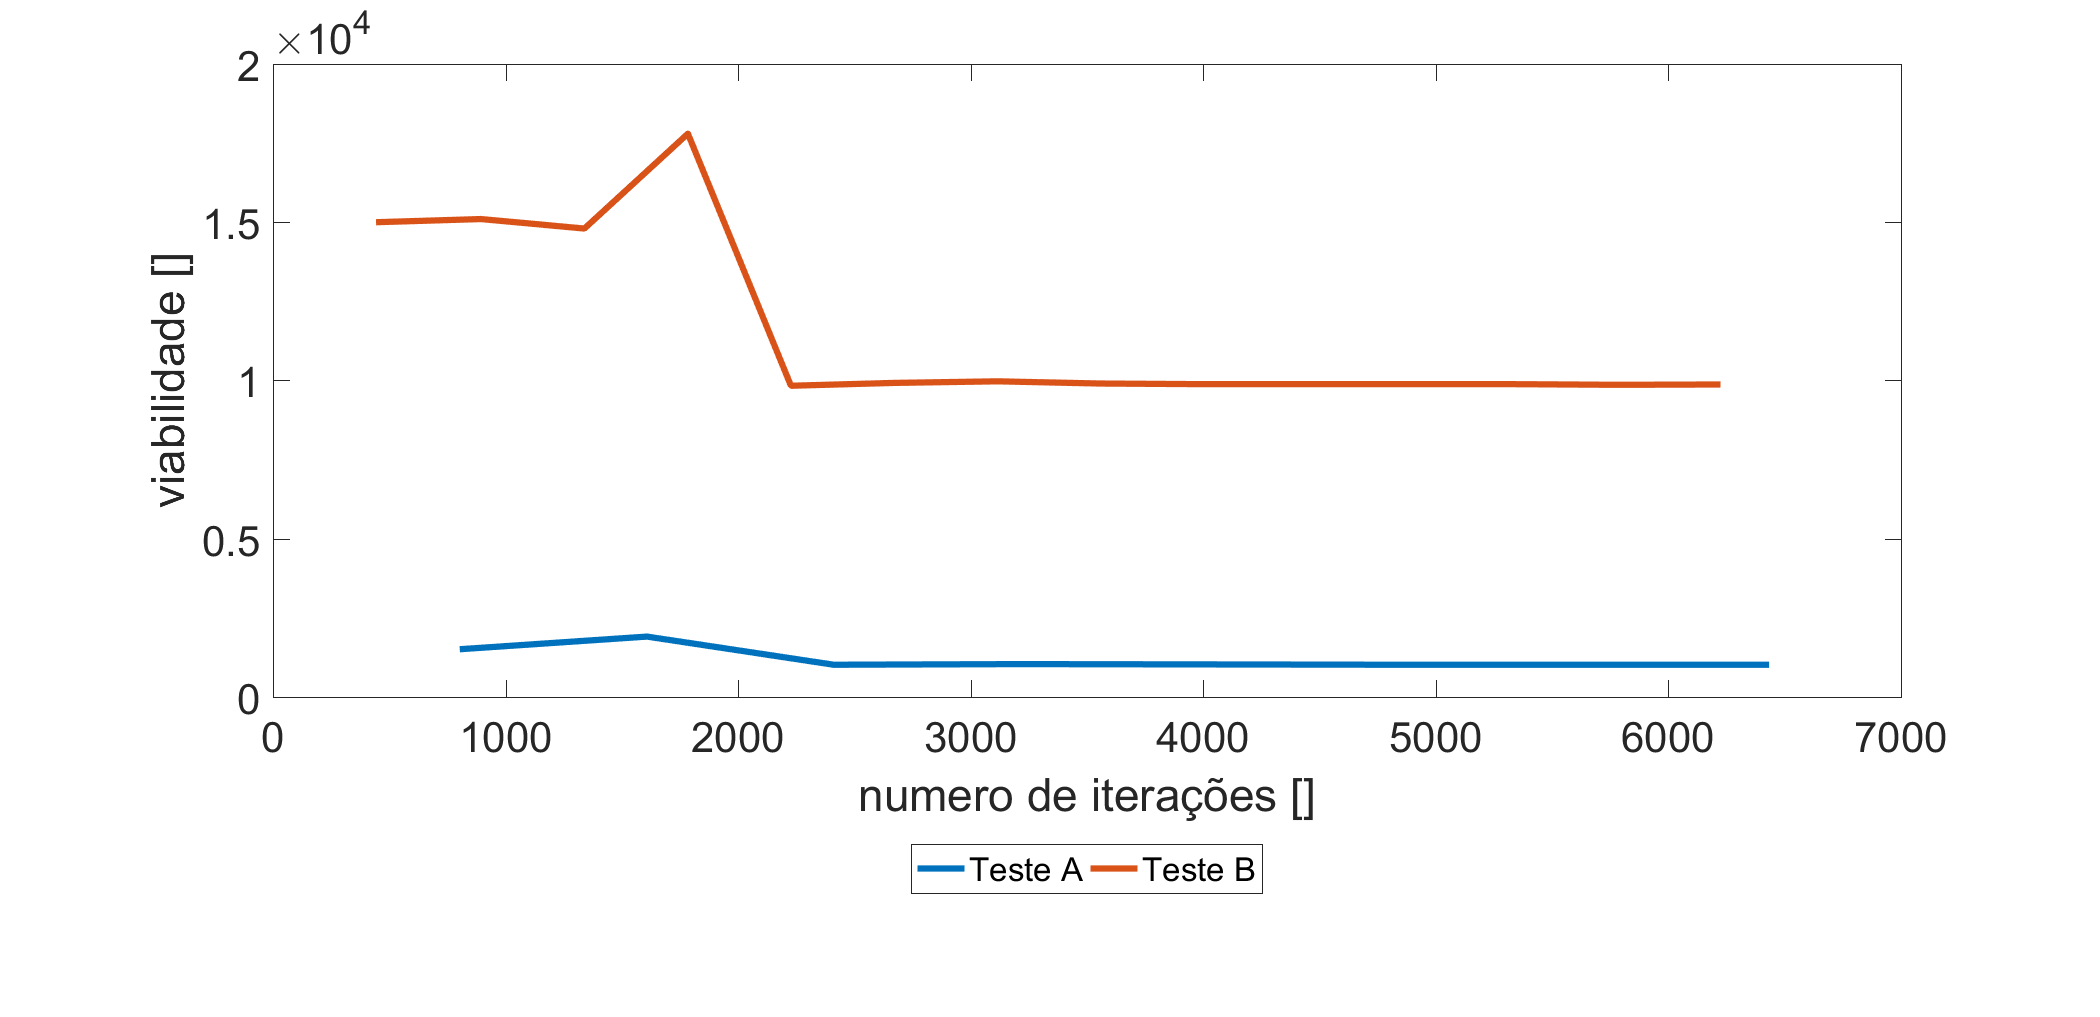
\includegraphics[scale=0.44]{Teste 3 Viabilidade}
    \label{fig:t_3_viab}
    \end{center}
\end{figure}

Uma possível explicação para as dificuldades observadas no Caso A pode ser encontrada no tamanho dos vetores de posição utilizados. No Caso A, o vetor de posições tinha 401 elementos e a simulação levou 195 segundos para ser concluída. Em contraste, o Caso B utilizou um vetor de 221 elementos e completou a simulação em 78 segundos. Estes resultados indicam que ajustes na aceleração podem ter implicações significativas não apenas no desempenho do sistema, mas também na eficiência computacional da simulação.

\subsection{Caso 4 - Variação dos passos de tempo}
Este caso destaca como diferentes resoluções na malha de tempo afetam o comportamento do sistema. As figuras \ref{fig:t_5a_vels}, \ref{fig:t_5b_vels} e \ref{fig:t_5c_vels} são fundamentais para entender a influência deste parâmetro nas oscilações observadas nos gráficos de velocidade. Cada uma destas figuras representa um cenário distinto, evidenciando como a resolução da malha de tempo pode alterar as dinâmicas de velocidade do sistema.

\begin{figure}[H]
    \begin{center}
    \caption{Caso 4A - Comportamento no tempo das velocidades em x e y da ponta e da referência}
    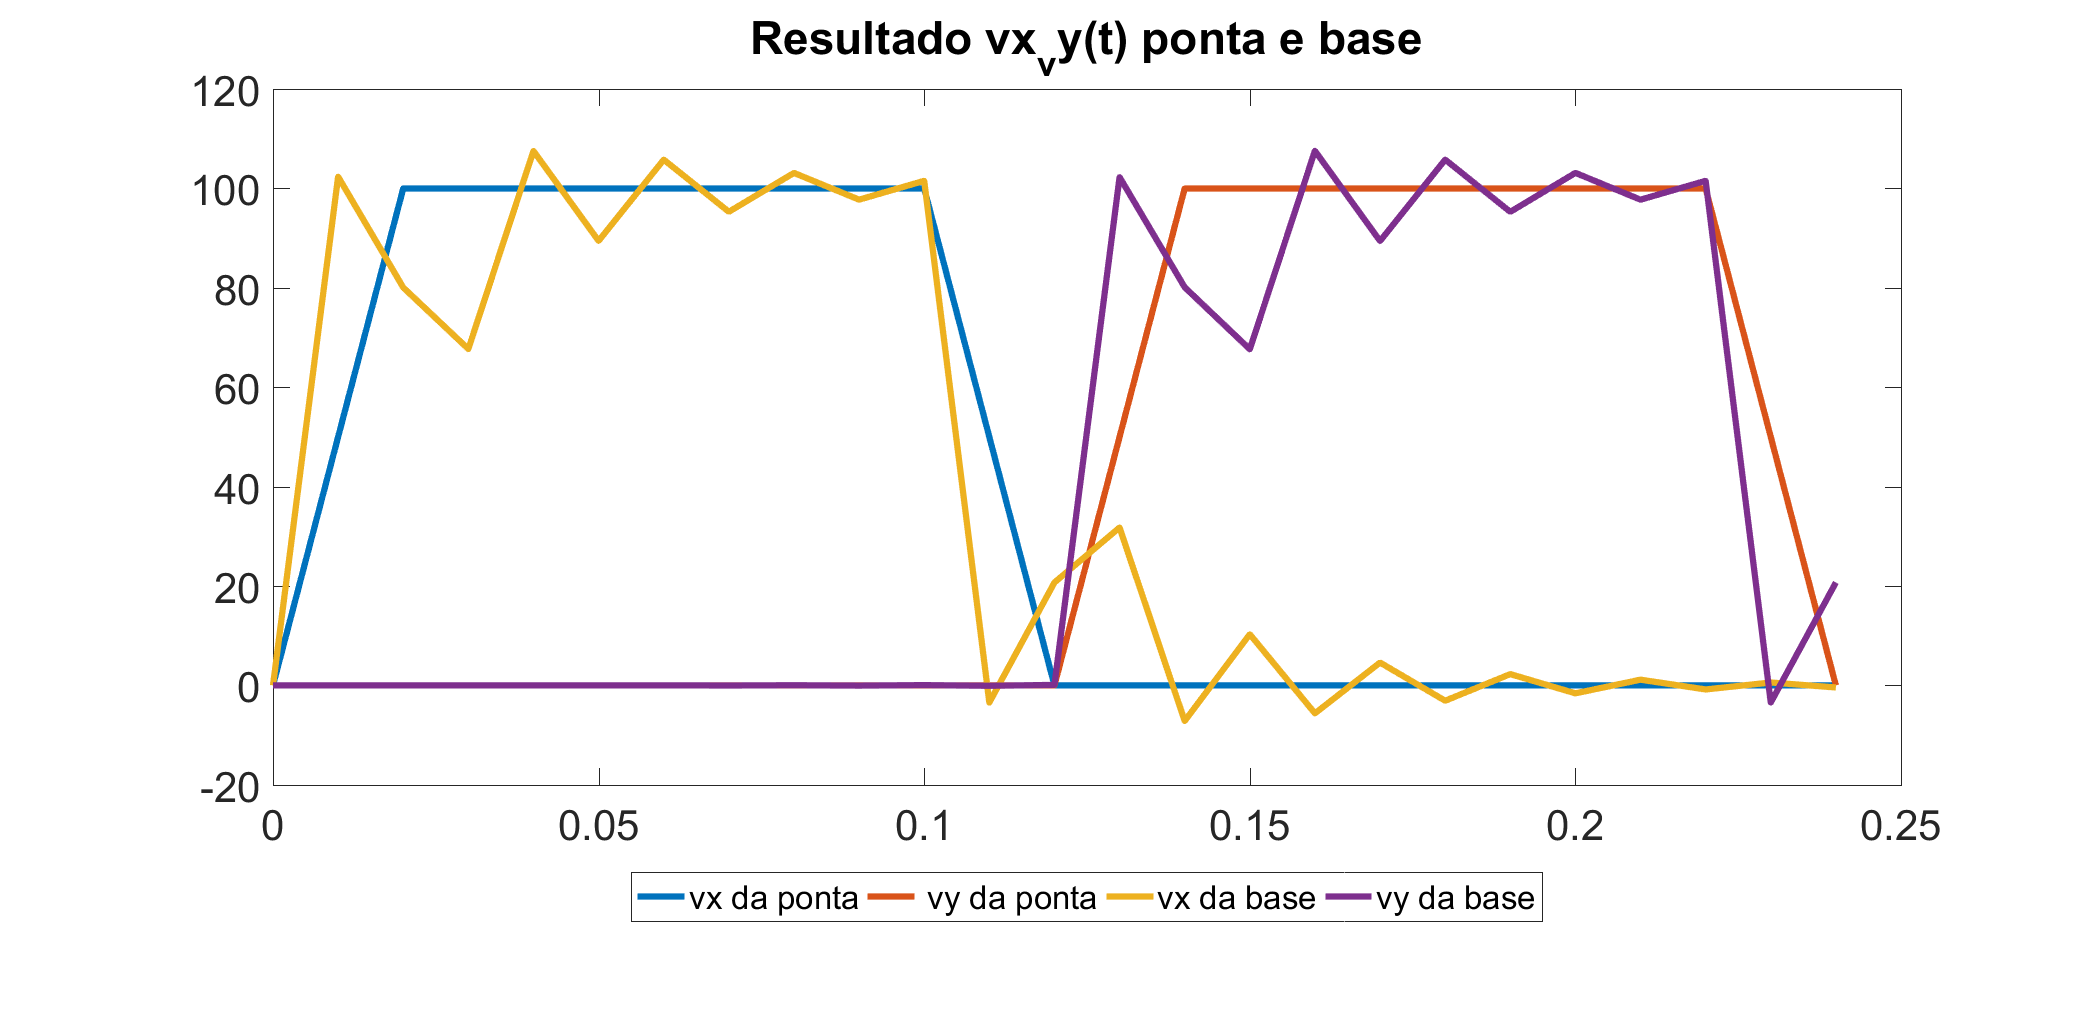
\includegraphics[scale=0.44]{Teste 5 A vels}
    \label{fig:t_5a_vels}
    \end{center}
\end{figure}

\begin{figure}[H]
    \begin{center}
    \caption{Caso 4B - Comportamento no tempo das velocidades em x e y da ponta e da referência}
    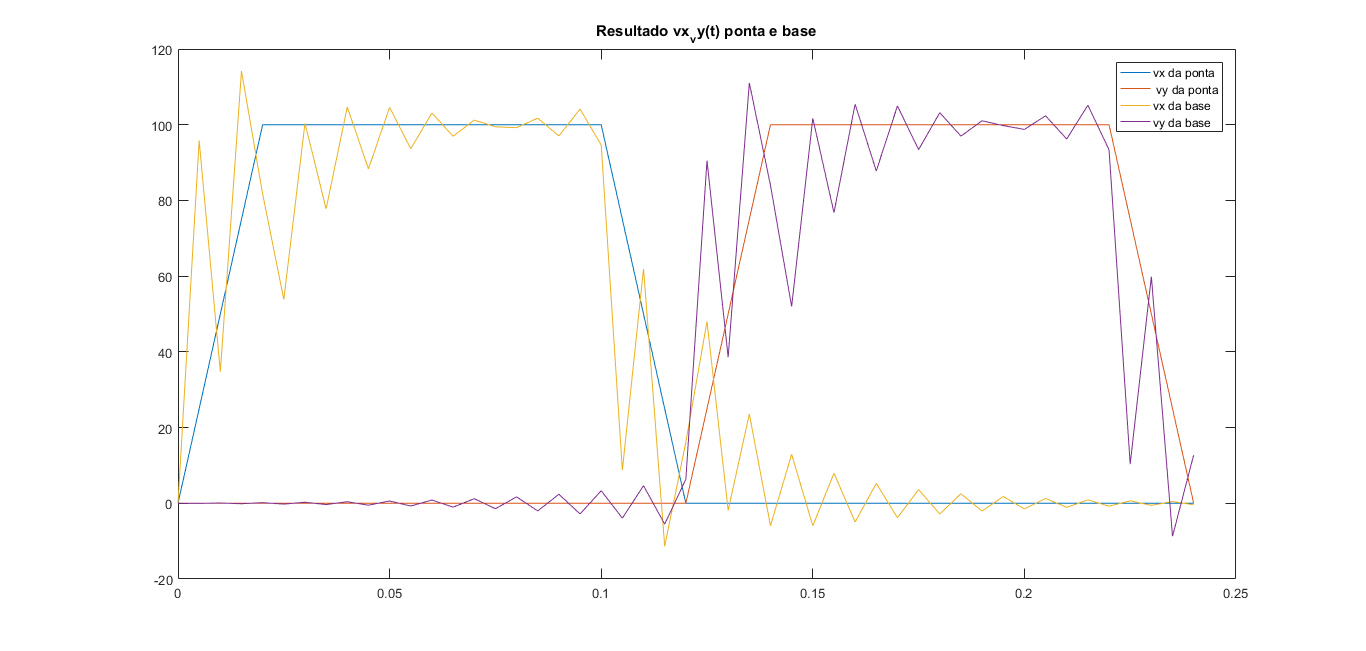
\includegraphics[scale=0.44]{Teste 5 B vels}
    \label{fig:t_5b_vels}
    \end{center}
\end{figure}

\begin{figure}[H]
    \begin{center}
    \caption{Caso 4C - Comportamento no tempo das velocidades em x e y da ponta e da referência}
    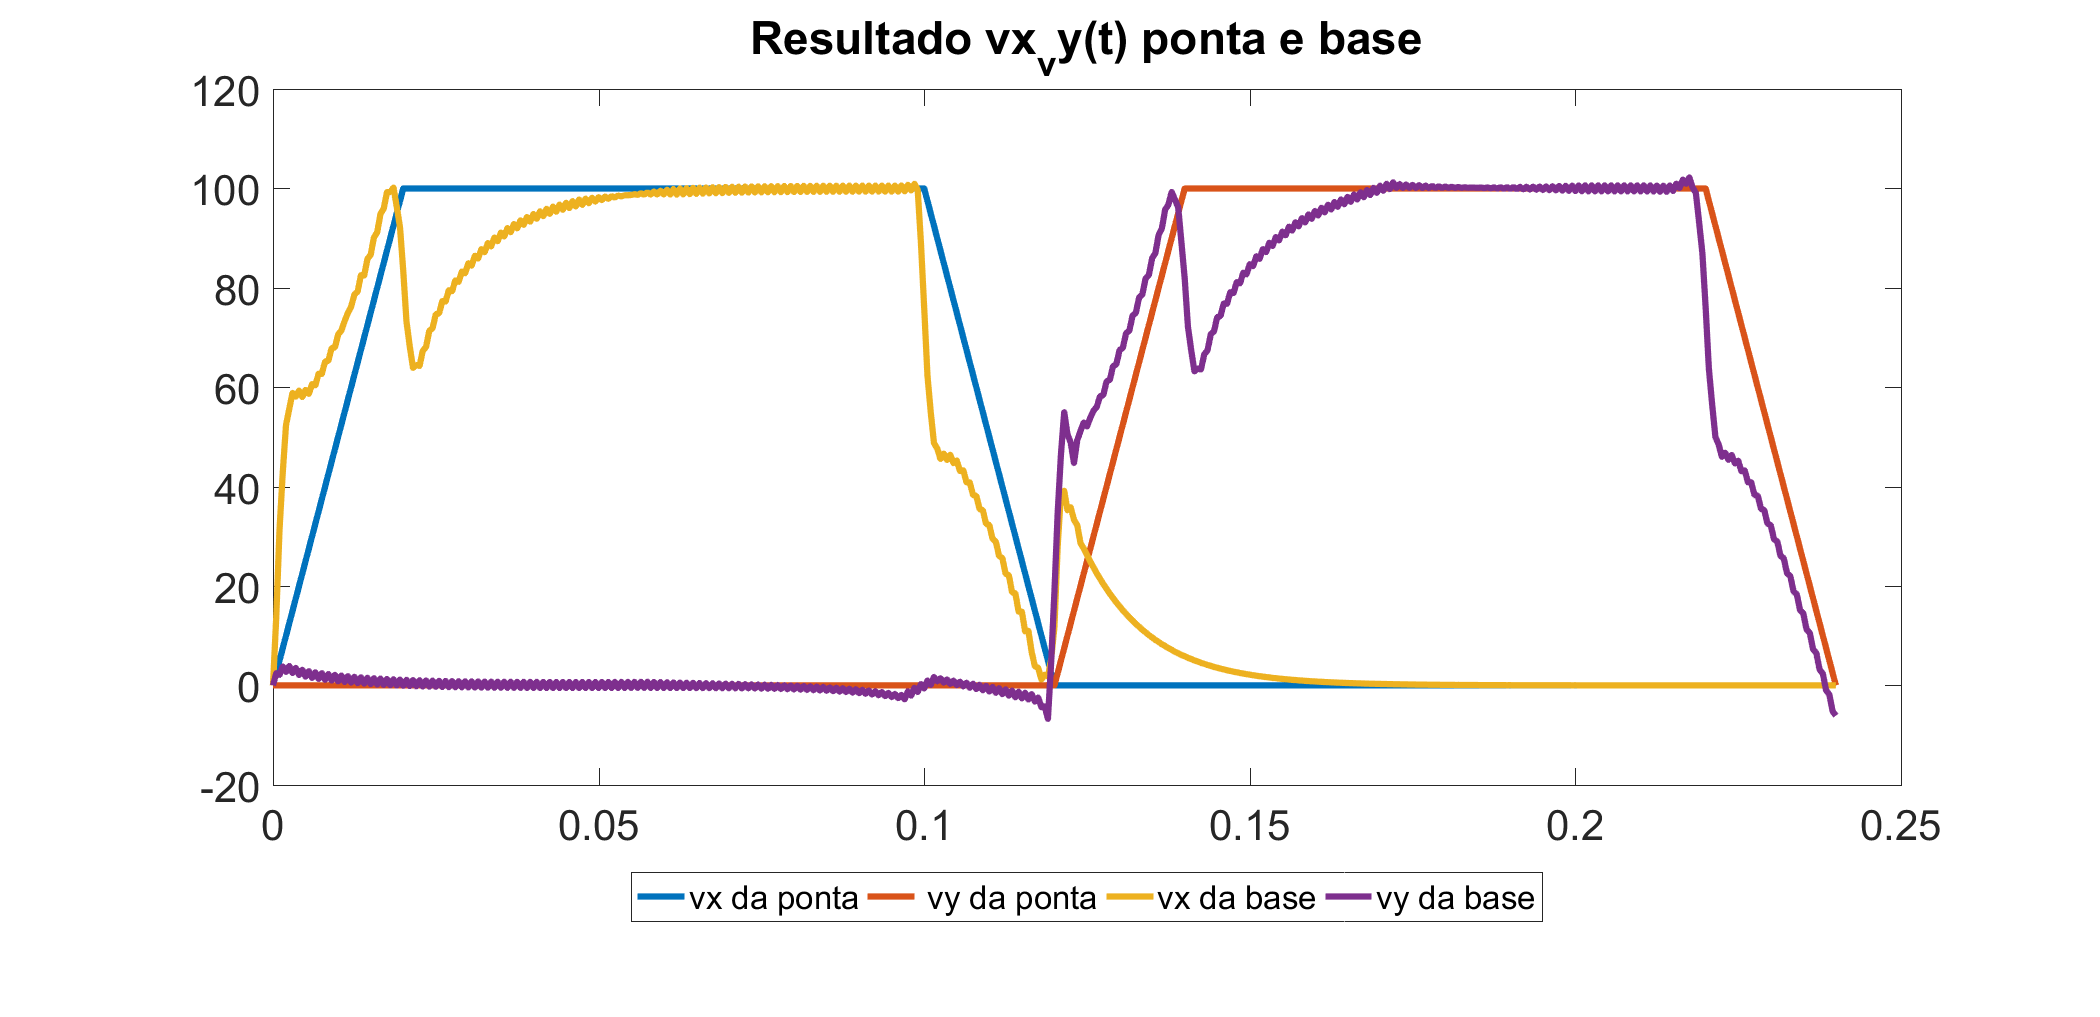
\includegraphics[scale=0.44]{Teste 5 C vels}
    \label{fig:t_5c_vels}
    \end{center}
\end{figure}

Por outro lado, ao examinar os gráficos de deslocamento nas figuras \ref{fig:t_5a_des}, \ref{fig:t_5b_des} e \ref{fig:t_5c_des}, notamos que as diferenças são menos pronunciadas. Isso sugere que, embora a resolução da malha de tempo tenha um impacto significativo na velocidade, seu efeito nos deslocamentos é mais sutil.

\begin{figure}[H]
    \begin{center}
    \caption{Caso 4A - Comportamento no tempo dos deslocamentos em x e y da ponta e da referência}
    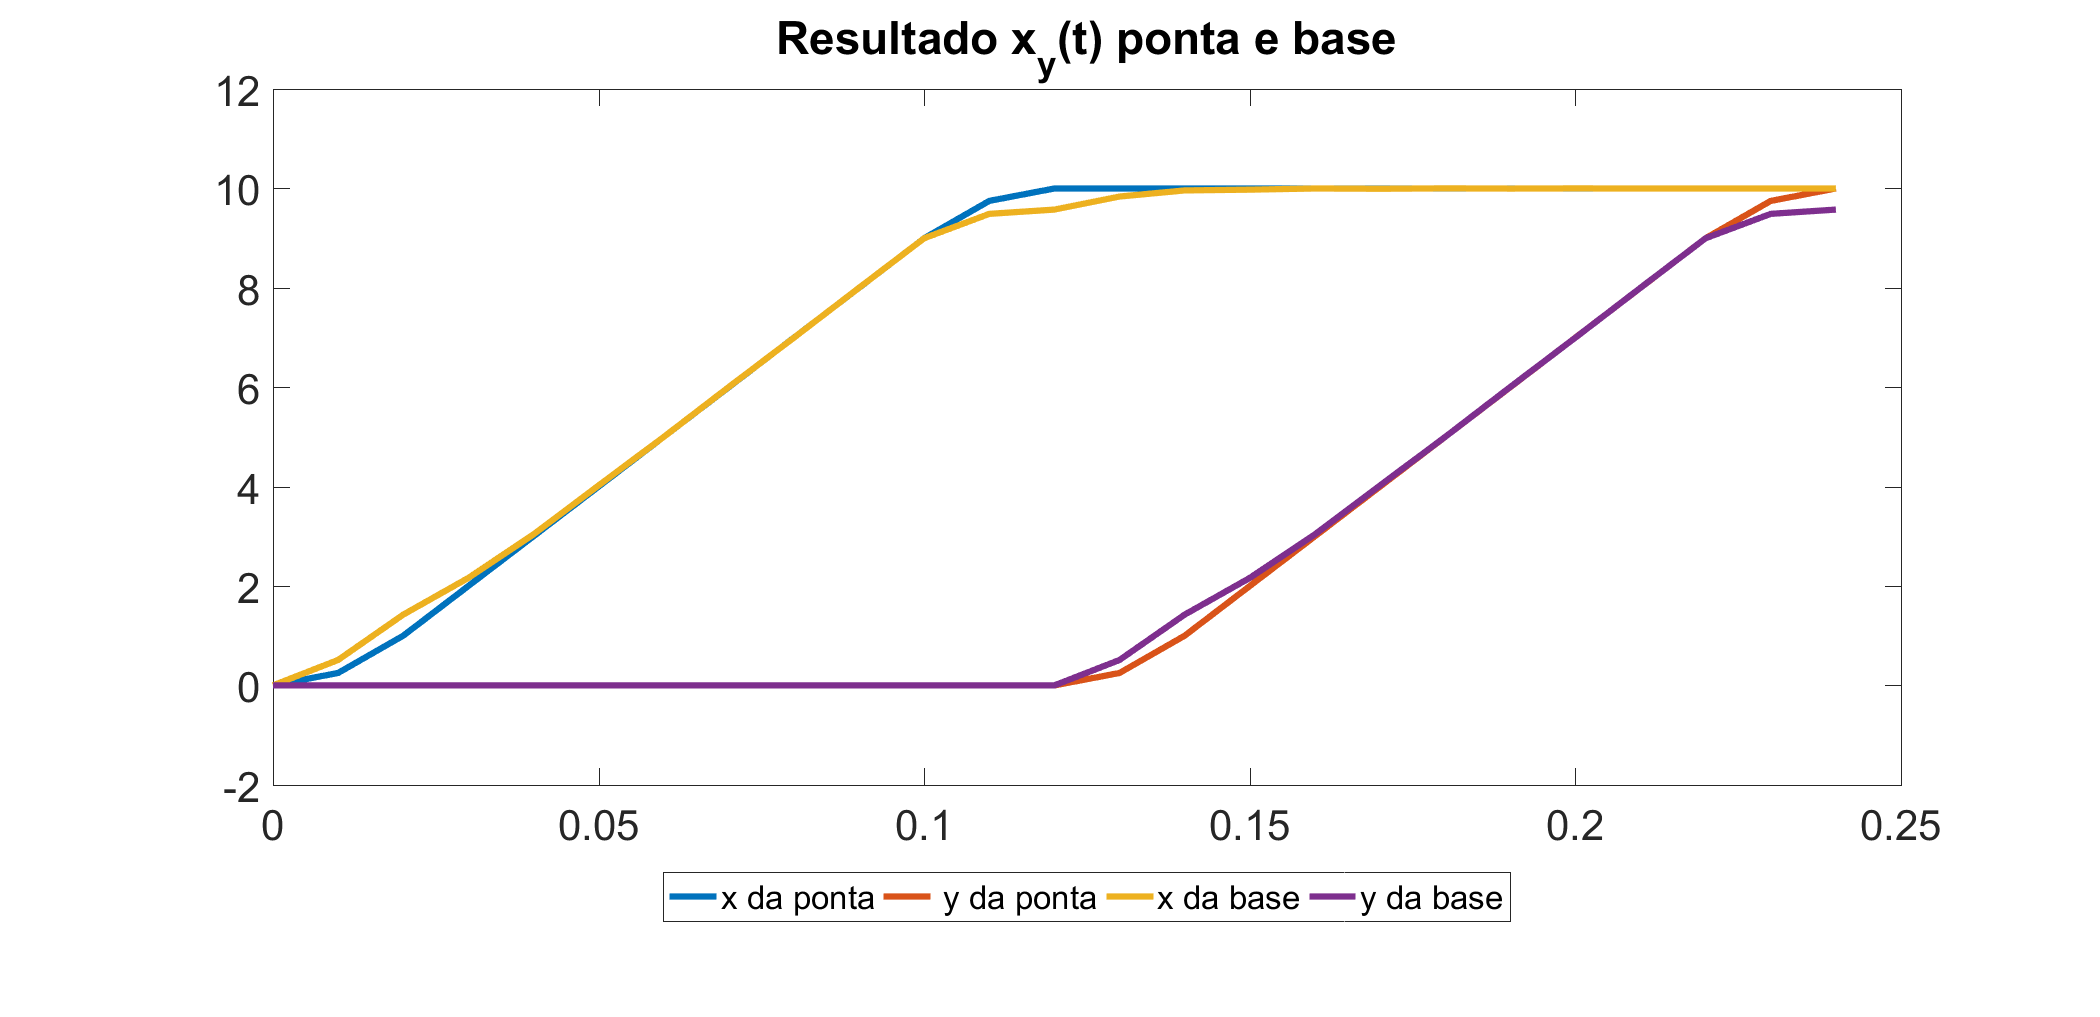
\includegraphics[scale=0.44]{Teste 5 A des}
    \label{fig:t_5a_des}
    \end{center}
\end{figure}

\begin{figure}[H]
    \begin{center}
    \caption{Caso 4B - Comportamento no tempo dos deslocamentos em x e y da ponta e da referência}
    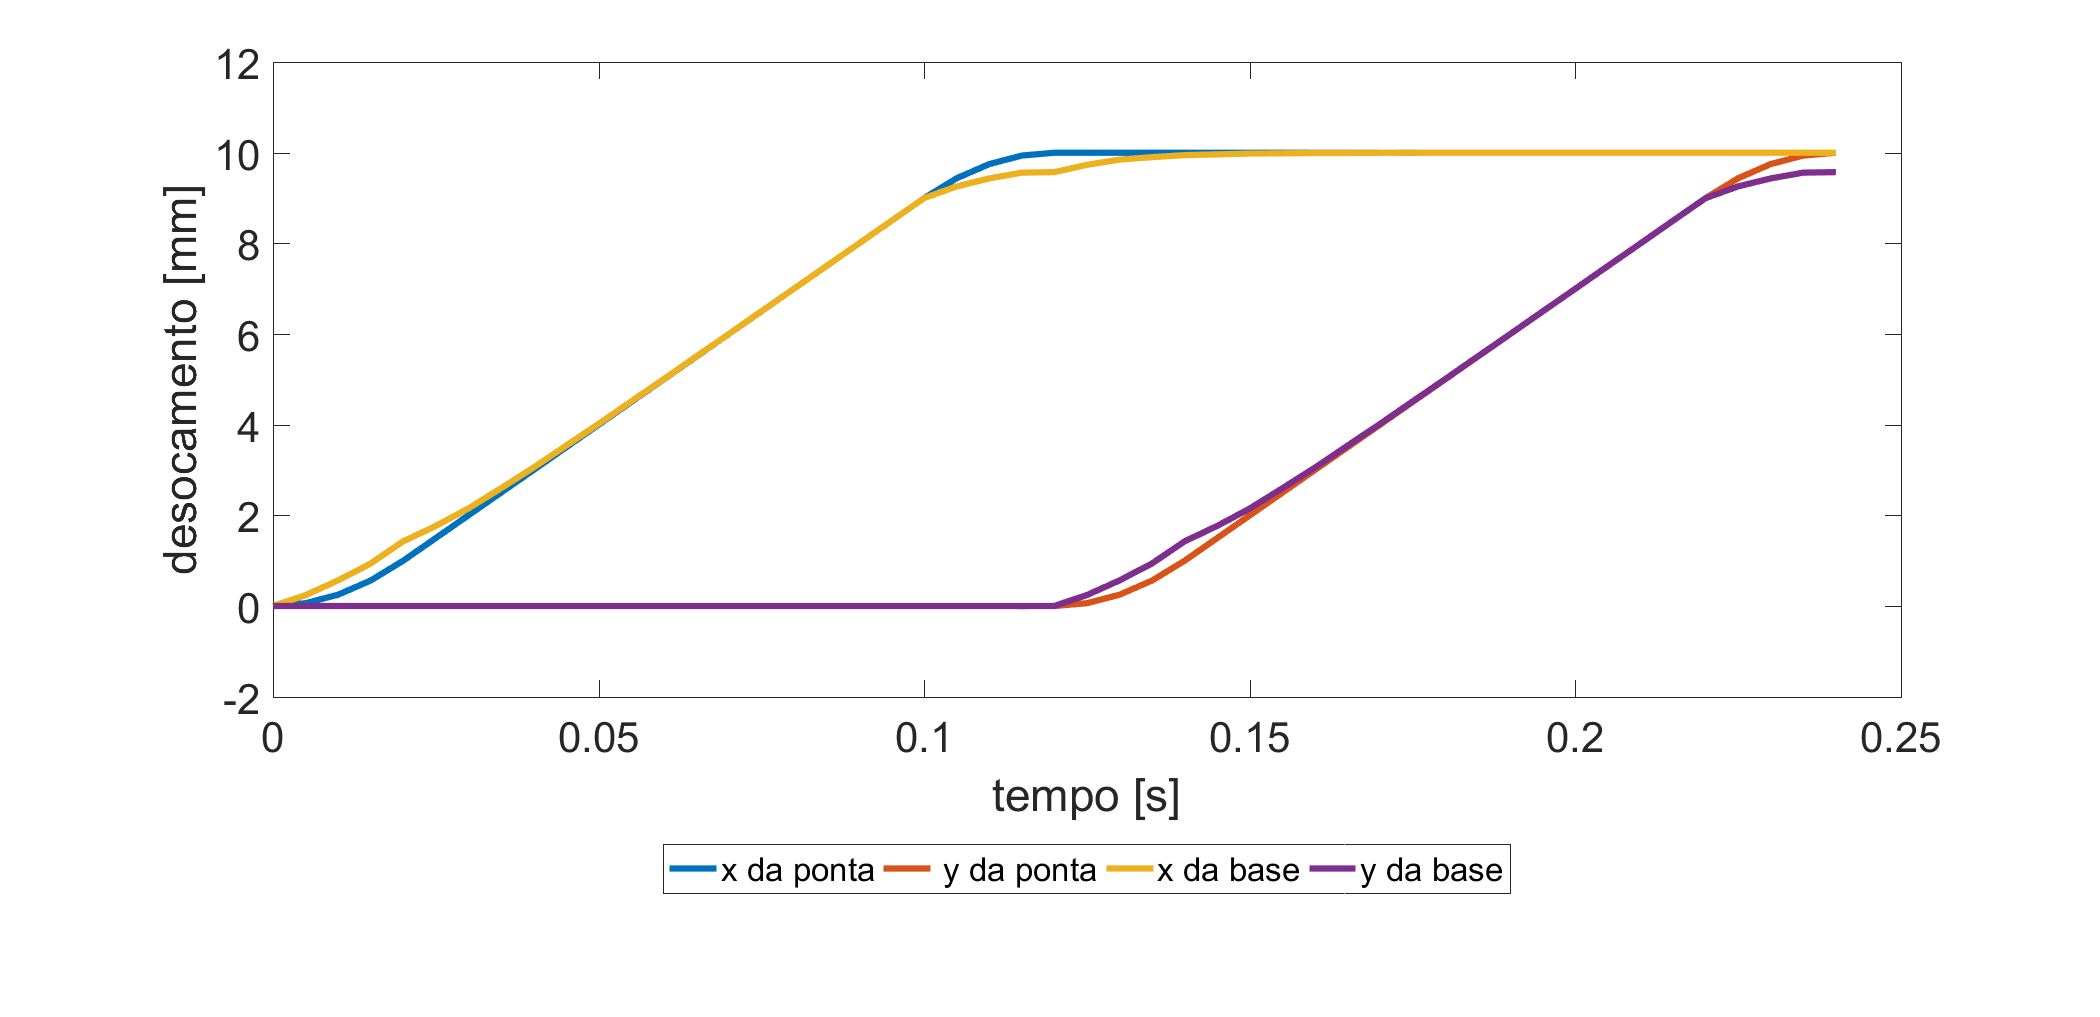
\includegraphics[scale=0.44]{Teste 5 B des}
    \label{fig:t_5b_des}
    \end{center}
\end{figure}

\begin{figure}[H]
    \begin{center}
    \caption{Caso 4C - Comportamento no tempo dos deslocamentos em x e y da ponta e da referência}
    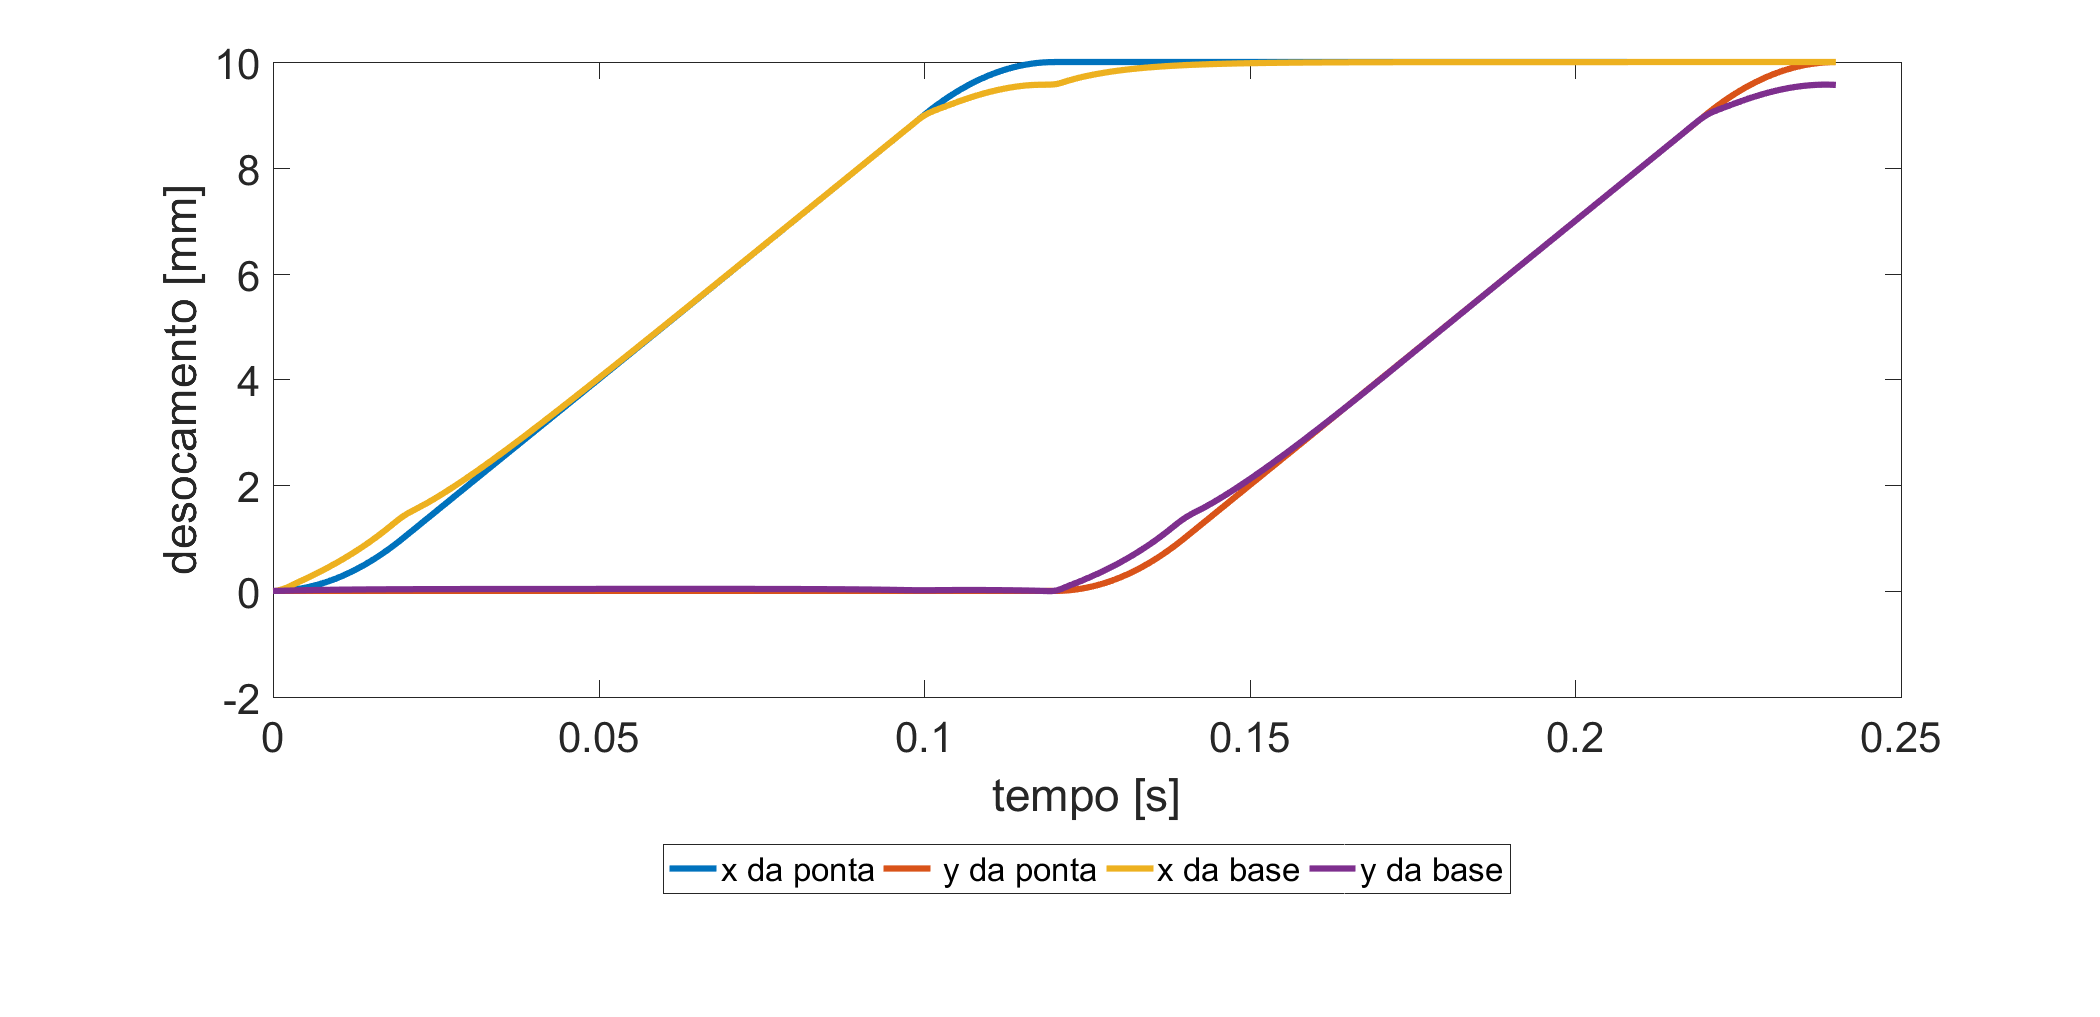
\includegraphics[scale=0.44]{Teste 5 C des}
    \label{fig:t_5c_des}
    \end{center}
\end{figure}

Além disso, a figura \ref{fig:t_5_viab} revela o impacto dessas variações na viabilidade da simulação, sugerindo uma relação entre a resolução da malha de tempo e a eficácia do sistema em alcançar a convergência. Os tempos de simulação variaram consideravelmente entre os casos, sendo 0,7 segundos para o Caso A, 3 segundos para o Caso B e 279 segundos para o Caso C. Este padrão de tempo está diretamente relacionado ao tamanho dos vetores de posição, que foram de 25, 49 e 481 elementos, respectivamente, para os Casos A, B e C.

\begin{figure}[H]
    \begin{center}
    \caption{Caso 4 - Num de fun x Viabilidade}
    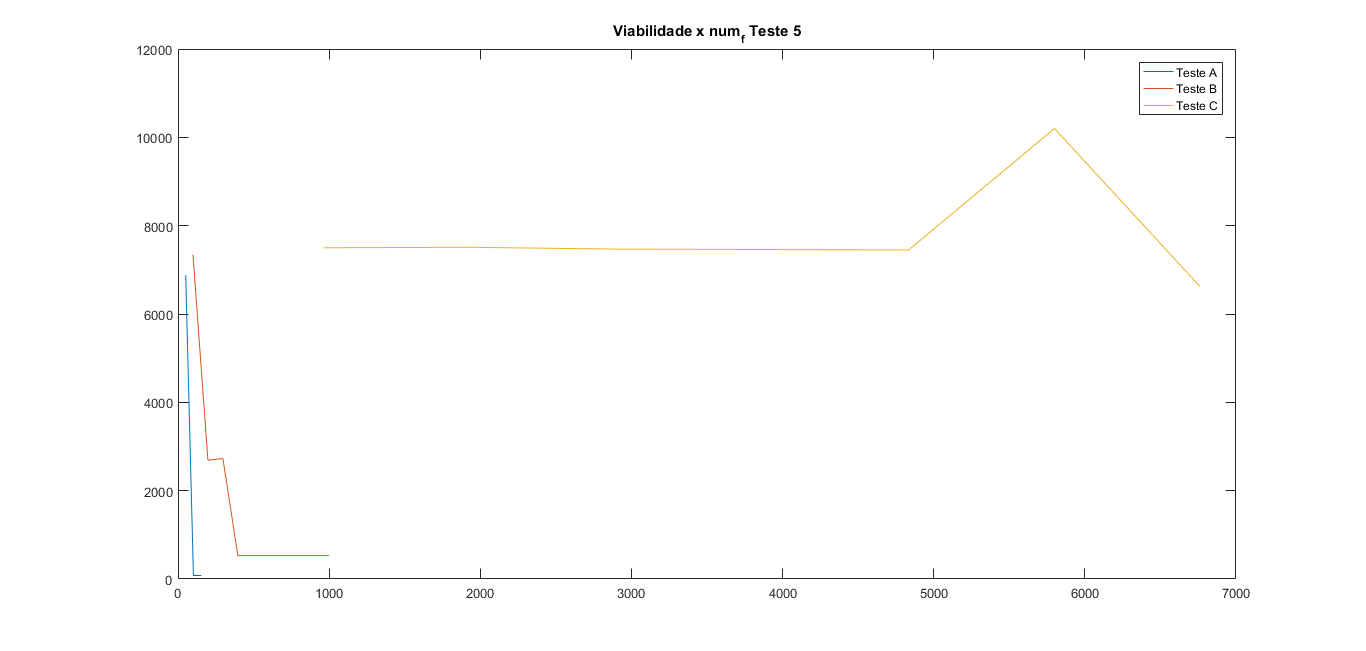
\includegraphics[scale=0.44]{Teste 5 Viabilidade}
    \label{fig:t_5_viab}
    \end{center}
\end{figure}

Podemos notar também o impacto na velocidade e facilidade de se convergir, podendo ser observado na figura \ref{fig:t_5_viab}, assim
como os tempos de simulação $0,7 s$, $3 s$ e $279 s$ para os Casos A, B e C respectivamente. Além do tamanho dos vetores que está diretamente relacionado,
respectivamente em 25, 49 e 481 para os Casos A, B e C.
\subsection{Caso 5 - Variação da velocidade}
Este caso foca na análise dos impactos causados por diferentes velocidades desejadas, ajustadas através do Gcode de entrada. Investigamos como as velocidades mais baixas e mais altas influenciam a dinâmica do sistema, tanto em termos de desempenho quanto de eficiência computacional.

No Caso A, onde a velocidade desejada é mais baixa, notamos um impacto significativo no tamanho dos vetores e no tempo de simulação. Devido à menor velocidade, o sistema leva mais tempo para completar o percurso, resultando em uma malha mais densa de pontos, dada a resolução de \(dt\) constante. Isso se traduz em um tempo de simulação mais longo de 219 segundos e 421 elementos nos vetores de posição.

Em contraste, o Caso B, com uma velocidade desejada mais alta, apresentou um tempo de simulação substancialmente menor de 60 segundos e 181 elementos nos vetores de posição. Interessante notar que, apesar da maior velocidade desejada e da manutenção da mesma aceleração máxima na geração de comando, a curva de velocidade neste caso assemelha-se à observada no Caso 3A, como mostrado na Figura \ref{fig:t_4b_vels}. A correspondente curva de deslocamento é ilustrada na Figura \ref{fig:t_4b_des}, destacando as diferenças no comportamento do sistema sob essas condições.

\begin{figure}[H]
    \begin{center}
    \caption{Caso 5B - Comportamento no tempo das velocidades em x e y da ponta e da referência}
    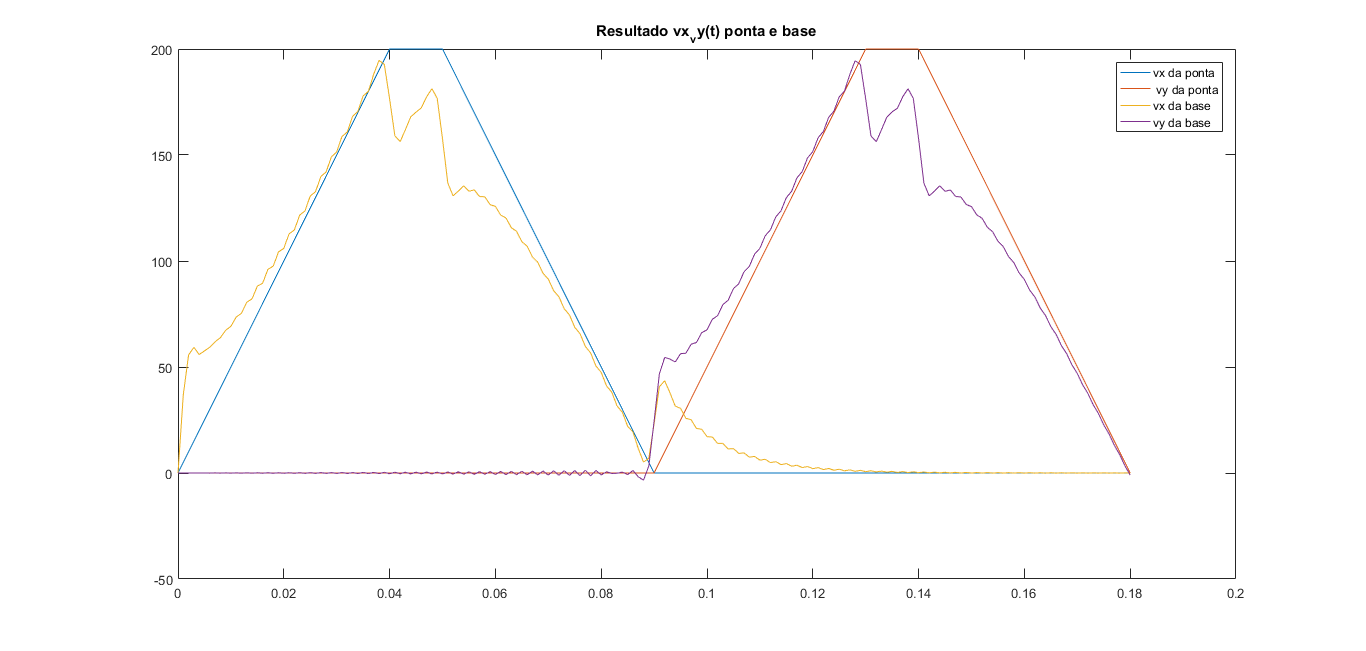
\includegraphics[scale=0.44]{Teste 4 B vels}
    \label{fig:t_4b_vels}
    \end{center}
\end{figure}

\begin{figure}[H]
    \begin{center}
    \caption{Caso 5B - Comportamento no tempo dos deslocamentos em x e y da ponta e da referência}
    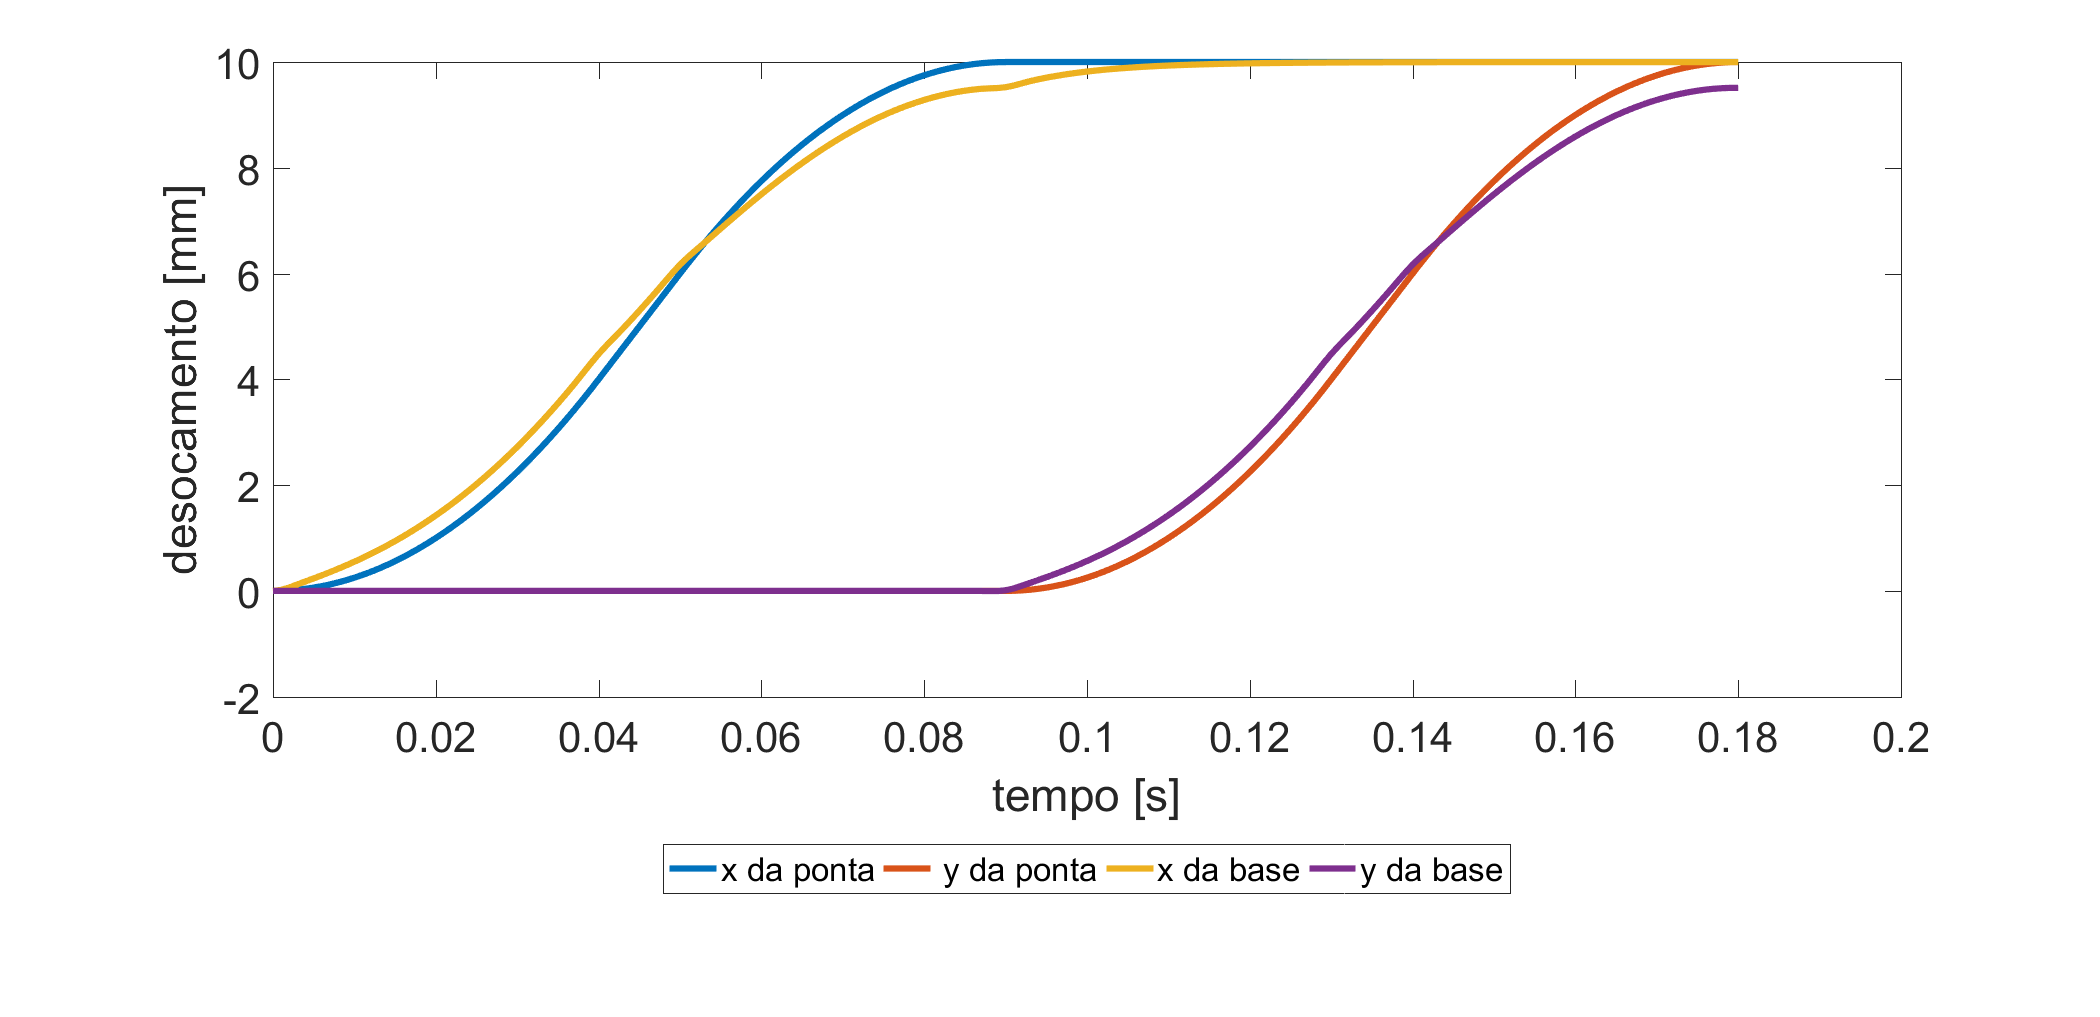
\includegraphics[scale=0.44]{Teste 4 B des}
    \label{fig:t_4b_des}
    \end{center}
\end{figure}

Além disso, a figura \ref{fig:t_4_viab} permite uma comparação do padrão de convergência em diferentes velocidades. Observa-se uma variação na viabilidade e na capacidade de o sistema atender às restrições impostas, variando de acordo com a velocidade configurada.

\begin{figure}[H]
    \begin{center}
    \caption{Caso 5 - Num de fun x Viabilidade}
    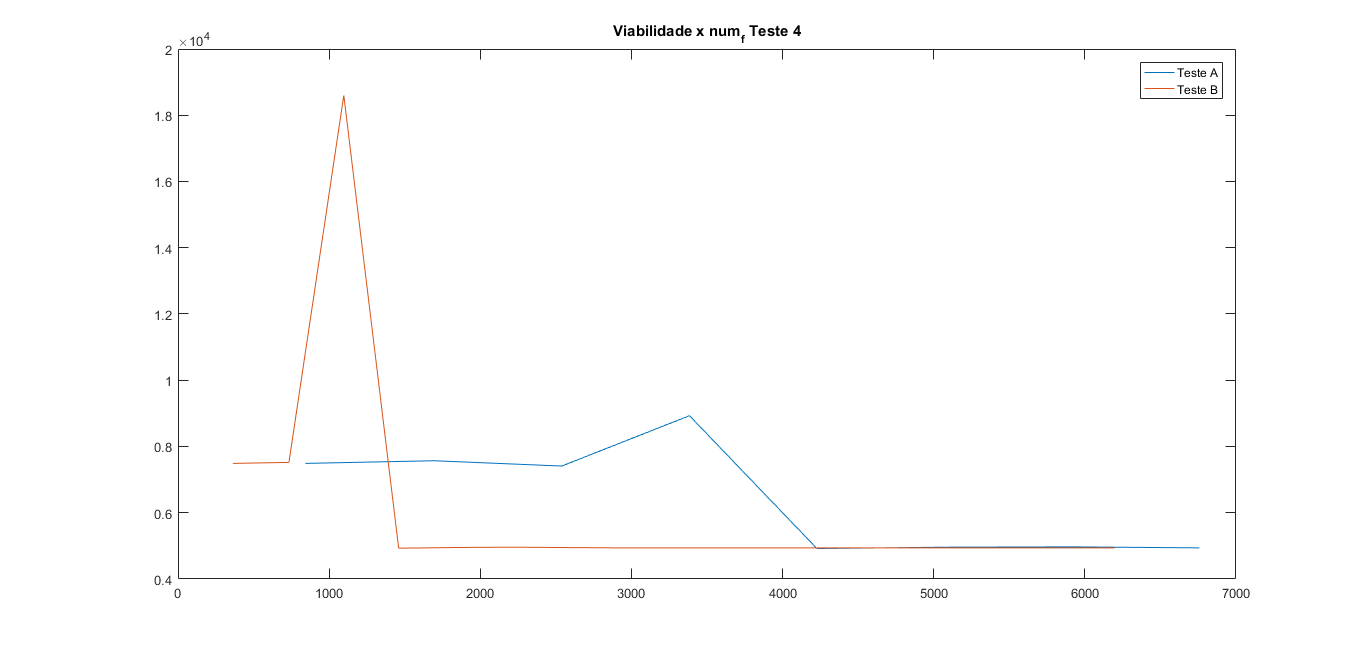
\includegraphics[scale=0.44]{Teste 4 Viabilidade}
    \label{fig:t_4_viab}
    \end{center}
\end{figure}

\section{Discussão Integrada dos Resultados}
Esta seção oferece uma análise integrada dos resultados obtidos nos diferentes casos de estudo, considerando as variáveis-chave e suas influências no comportamento do sistema simulado. A discussão foca em identificar padrões comuns, divergências e as implicações práticas dos resultados obtidos.

\subsection{Influência dos Parâmetros Variáveis}
A análise de sensibilidade realizada nos Casos 1 a 5 revelou que variações em parâmetros específicos, como frequência natural, coeficiente de amortecimento, aceleração, resolução de malha de tempo e velocidade desejada, têm impactos significativos e distintos no comportamento do sistema. 

No Caso 1, observou-se que a variação da frequência natural afeta diretamente a amplitude dos desvios e a necessidade de compensação. O Caso 2 mostrou que diferentes coeficientes de amortecimento podem levar a variações notáveis na trajetória e na viabilidade do sistema. No Caso 3, a alteração da aceleração demonstrou como esse parâmetro pode influenciar a forma da curva de velocidade e a eficiência da simulação. O Caso 4 destacou a importância da resolução da malha de tempo, especialmente em relação às oscilações de velocidade. Por fim, o Caso 5 ilustrou como a velocidade desejada afeta tanto o tempo de simulação quanto o tamanho dos vetores de posição.

\subsection{Comportamento e Convergência do Sistema}
Em todos os casos, observou-se uma tendência de convergência para soluções viáveis, embora com variações na velocidade e facilidade desta convergência. Notavelmente, os casos com maiores desafios em termos de convergência e viabilidade foram aqueles com maiores variações nos parâmetros estudados. Isso sugere que, enquanto o sistema é robusto e adaptável a uma ampla gama de condições, existem limites críticos além dos quais a eficácia do sistema começa a diminuir.

\subsection{Considerações futuras}
Uma possível abordagem a ser explorada utilizando a ideia do método deste trabalho é a sobreposição de algoritmos, onde
um método referenciado em uma planta do sistema poderia buscar remover uma parcela das vibrações, atuando de forma estagiada,
com a participação de um método como \textit{InputShaping} para atacar as vibrações remanescentes.

Uma possibilidade que o tipo de método abordado neste trabalho oferece é a capacidade de otimizar os parâmetros da planta para uma determinada posição.
Assim, oferecendo a capacidade de se ajustar em grande nível de detalhe as peculiaridades do sistema, podendo até
construir a malha utilizando sensores, semelhantemente a rotinas de configuração de \textit{InputShaping} que amostram
o comportamento em frequência no ponto central da impressora. Considerando também que a utilização desse tipo de malha,
teria pouco impacto computacional.


